\documentclass[conference]{IEEEtran}
\IEEEoverridecommandlockouts
% The preceding line is only needed to identify funding in the first footnote. If that is unneeded, please comment it out.
%Template version as of 6/27/2024

\usepackage{cite}
\usepackage{amsmath,amssymb,amsfonts}
%\usepackage{algorithmic}
\usepackage{graphicx}
\usepackage{textcomp}
\usepackage{xcolor}
\def\BibTeX{{\rm B\kern-.05em{\sc i\kern-.025em b}\kern-.08em
    T\kern-.1667em\lower.7ex\hbox{E}\kern-.125emX}}
% Common packages
\usepackage[utf8]{inputenc} % allow utf-8 input
\usepackage[T1]{fontenc}    % use 8-bit T1 fonts
\usepackage{microtype,inconsolata}
\usepackage{times,latexsym}
\usepackage{graphicx} \graphicspath{{figures/}}
\usepackage{amsmath,amssymb,mathabx,mathtools,amsthm,nicefrac}
% \usepackage{algorithmic}
\usepackage[linesnumbered,ruled,vlined]{algorithm2e}
\usepackage{acronym}
\usepackage{enumitem}
%\usepackage[pagebackref,breaklinks,colorlinks]{hyperref}
\usepackage{balance}
\usepackage{xspace}
\usepackage{setspace}
\usepackage[skip=3pt,font=small]{subcaption}
\usepackage[skip=3pt,font=small]{caption}
%\usepackage[dvipsnames,svgnames,x11names,table]{xcolor}
\usepackage[capitalise,noabbrev,nameinlink]{cleveref}
\usepackage{booktabs,tabularx,colortbl,multirow,multicol,array,makecell,tabularray}
\usepackage{overpic,wrapfig}
\usepackage[misc]{ifsym}
\usepackage{pifont}
\usepackage{diagbox}


% Handy shorthand
\makeatletter
\DeclareRobustCommand\onedot{\futurelet\@let@token\@onedot}
\def\@onedot{\ifx\@let@token.\else.\null\fi\xspace}
\def\eg{\emph{e.g}\onedot} 
\def\Eg{\emph{E.g}\onedot}
\def\ie{\emph{i.e}\onedot} 
\def\Ie{\emph{I.e}\onedot}
\def\cf{\emph{c.f}\onedot} 
\def\Cf{\emph{C.f}\onedot}
\def\etc{\emph{etc}\onedot} 
\def\vs{\emph{vs}\onedot}
\def\aka{a.k.a\onedot}
\def\wrt{w.r.t\onedot} 
\def\dof{d.o.f\onedot}
\def\etal{\emph{et al}\onedot}
\makeatother

% Handy math ops
%\DeclareMathOperator*{\argmax}{arg\,max}
%\DeclareMathOperator*{\argmin}{arg\,min}
\DeclareMathOperator*{\kl}{KL}
\newcommand\energy{\mathcal{E}}
\newcommand{\norm}[1]{\left\Vert #1 \right\Vert}

% Handy table symbols
\newcommand{\cmark}{\ding{51}}%
\newcommand{\xmark}{\ding{55}}%

% Spacing
\frenchspacing
\makeatletter
\renewcommand{\paragraph}{%
  \@startsection{paragraph}{4}%
  {\z@}{0ex \@plus 0ex \@minus 0ex}{-1em}%
  {\hskip0em\normalfont\normalsize\bfseries}%
}
\makeatother

% Clever references
\crefname{algorithm}{Alg.}{Algs.}
\Crefname{algocf}{Algorithm}{Algorithms}
\crefname{section}{Sec.}{Secs.}
\Crefname{section}{Section}{Sections}
\crefname{table}{Tab.}{Tabs.}
\Crefname{table}{Table}{Tables}
\crefname{figure}{Fig.}{Figs.}
\Crefname{figure}{Figure}{Figures}
\crefname{equation}{Eq.}{Eqs.}
\Crefname{equation}{Equation}{Equations}
\crefname{appendix}{Appx.}{Appxs.}
\Crefname{appendix}{Appendix}{Appendices}

% Handy Colors
\definecolor{gblue}{HTML}{4285F4}
\definecolor{gred}{HTML}{DB4437}
\definecolor{ggreen}{HTML}{0F9D58}

\hypersetup{
  %citecolor=gray %Colour of citations
}

% Spacing
% \frenchspacing
% \medmuskip=2mu   % reduce spacing around binary operators
% \thickmuskip=3mu % reduce spacing around relational operators
% \setlength{\abovedisplayskip}{3pt}
% \setlength{\belowdisplayskip}{3pt}
% \setlength{\abovecaptionskip}{3pt}
% \setlength{\belowcaptionskip}{3pt}
% \setlength\floatsep{0.5\baselineskip plus 3pt minus 2pt}
% \setlength\textfloatsep{0.5\baselineskip plus 3pt minus 2pt}
% \setlength\dbltextfloatsep{0.5\baselineskip plus 3pt minus 2pt}
% \setlength\intextsep{0.5\baselineskip plus 3pt minus 2pt}

\newcolumntype{P}[1]{>{\centering\arraybackslash}p{#1}}
\newcolumntype{M}[1]{>{\centering\arraybackslash}m{#1}}

\acrodef{metaicl-w}[Minnow]{Meta-training for IN-context learNing Of Words}
\acrodef{metaicl}[MetaICL]{Meta-training for In-Context Learning}
\acrodef{icl}[ICL]{in-context learning}
\author{%
  Wentao Wang$^1$ \hspace{1em} Guangyuan Jiang$^2$ \hspace{1em} Tal Linzen$^1$ \hspace{1em} Brenden M.\ Lake$^1$ \\
  $^1$New York University \hspace{1em} $^2$Peking University \\
  \texttt{\{ww2135, linzen, brenden\}@nyu.edu} \hspace{1em} \texttt{jgy@stu.pku.edu.cn}
}
\begin{document}

%\title{Systolic Xtreme: Selecting Low-Critical-Delay Weights for Accelerating LLM Inference}
\title{HALO: \underline{H}ardware-\underline{a}ware quantization with \underline{lo}w critical-path-delay weights for LLM acceleration}

\begin{comment}
\author{\IEEEauthorblockN{Rohan Juneja}
\IEEEauthorblockA{\textit{School of Computing} \\
\textit{National University of Singapore}\\
rohan@comp.nus.edu.sg}
\and
\IEEEauthorblockN{Shivam Aggarwal}
\IEEEauthorblockA{\textit{School of Computing} \\
\textit{National University of Singapore}\\
shivam@comp.nus.edu.sg}
\and
\IEEEauthorblockN{Safeen Huda}
\IEEEauthorblockA{\textit{Google}\\
safeen@google.com}
\and
\IEEEauthorblockN{Tulika Mitra}
\IEEEauthorblockA{\textit{School of Computing} \\
\textit{National University of Singapore}\\
tulika@comp.nus.edu.sg}
\and
\IEEEauthorblockN{Li-Shiuan Peh}
\IEEEauthorblockA{\textit{School of Computing} \\
\textit{National University of Singapore}\\
peh@comp.nus.edu.sg}
}
\end{comment}

\author{
    \IEEEauthorblockN{
        Rohan Juneja\IEEEauthorrefmark{1},
        Shivam Aggarwal\IEEEauthorrefmark{1},
        Safeen Huda\IEEEauthorrefmark{2}
        Tulika Mitra\IEEEauthorrefmark{1},
        Li-Shiuan Peh\IEEEauthorrefmark{1},
    }
    \\
    \IEEEauthorblockA{\IEEEauthorrefmark{1}School of Computing, National University of Singapore, \IEEEauthorrefmark{2}Google\\ 
    \{rohan, shivam, tulika, peh\}@comp.nus.edu.sg, 
    safeen@google.com}
}

\maketitle

\begin{comment}
\begin{abstract}
The rapid expansion of Transformer-based models has significantly outpaced advancements in hardware, leading to increased inference costs.
To address the gap between growing model sizes and hardware limitations, model quantization presents a promising solution. 
However, current quantization techniques do not account for the critical path variations in Multiply-Accumulate (MAC) operations, which differ significantly with each weight value due to the iterative shift-add architecture of MAC units.
This paper introduces Systolic Xtreme (SystolicX), a novel hardware-software co-design aimed at accelerating models on Systolic Arrays by leveraging unique frequency scaling opportunities.

SystolicX capitalizes on the relationship between weight values and their effective critical path timing at runtime. 
It proposes a Hardware-Aware Post-Training quantization framework that incorporates hardware accelerator timing and power analysis. 
This framework strategically quantizes model weights, prioritizing those with lower critical delay, thereby reducing the circuit's overall critical delay. 
This reduction enables dynamic frequency adjustment to higher clock frequencies, achieving significant performance and energy improvements.
SystolicX demonstrates the potential to deliver up to ?? times speedup and ?? power savings, all without compromising accuracy and with minimal area overhead.
\end{abstract}
\end{comment}

\begin{abstract}
%Cambrian explosion of accelerators for LLMs has fragmented the hardware landscape, highlighting the need to optimize existing platforms over developing bespoke solutions. 
Quantization is critical for realizing efficient inference of LLMs.
Traditional quantization methods are hardware-agnostic, limited to bit-width constraints, and lacking circuit-level insights, such as timing and energy characteristics of Multiply-Accumulate (MAC) units. We introduce \textit{HALO}, a versatile framework that adapts to various hardware through a Hardware-Aware Post-Training Quantization (PTQ) approach. By leveraging MAC unit properties, \textit{HALO} minimizes critical-path delays and enables dynamic frequency scaling. Deployed on LLM accelerators like TPUs and GPUs, \textit{HALO} achieves on average 270\% performance gains and 51\% energy savings, all with minimal accuracy drop.
%{\bf Peh: Why is there area overhead?}
\end{abstract}
\begin{IEEEkeywords}
LLMs, Quantization, DVFS, TPUs, GPUs
\end{IEEEkeywords}

\section{Introduction}
\label{sec:introduction}
The business processes of organizations are experiencing ever-increasing complexity due to the large amount of data, high number of users, and high-tech devices involved \cite{martin2021pmopportunitieschallenges, beerepoot2023biggestbpmproblems}. This complexity may cause business processes to deviate from normal control flow due to unforeseen and disruptive anomalies \cite{adams2023proceddsriftdetection}. These control-flow anomalies manifest as unknown, skipped, and wrongly-ordered activities in the traces of event logs monitored from the execution of business processes \cite{ko2023adsystematicreview}. For the sake of clarity, let us consider an illustrative example of such anomalies. Figure \ref{FP_ANOMALIES} shows a so-called event log footprint, which captures the control flow relations of four activities of a hypothetical event log. In particular, this footprint captures the control-flow relations between activities \texttt{a}, \texttt{b}, \texttt{c} and \texttt{d}. These are the causal ($\rightarrow$) relation, concurrent ($\parallel$) relation, and other ($\#$) relations such as exclusivity or non-local dependency \cite{aalst2022pmhandbook}. In addition, on the right are six traces, of which five exhibit skipped, wrongly-ordered and unknown control-flow anomalies. For example, $\langle$\texttt{a b d}$\rangle$ has a skipped activity, which is \texttt{c}. Because of this skipped activity, the control-flow relation \texttt{b}$\,\#\,$\texttt{d} is violated, since \texttt{d} directly follows \texttt{b} in the anomalous trace.
\begin{figure}[!t]
\centering
\includegraphics[width=0.9\columnwidth]{images/FP_ANOMALIES.png}
\caption{An example event log footprint with six traces, of which five exhibit control-flow anomalies.}
\label{FP_ANOMALIES}
\end{figure}

\subsection{Control-flow anomaly detection}
Control-flow anomaly detection techniques aim to characterize the normal control flow from event logs and verify whether these deviations occur in new event logs \cite{ko2023adsystematicreview}. To develop control-flow anomaly detection techniques, \revision{process mining} has seen widespread adoption owing to process discovery and \revision{conformance checking}. On the one hand, process discovery is a set of algorithms that encode control-flow relations as a set of model elements and constraints according to a given modeling formalism \cite{aalst2022pmhandbook}; hereafter, we refer to the Petri net, a widespread modeling formalism. On the other hand, \revision{conformance checking} is an explainable set of algorithms that allows linking any deviations with the reference Petri net and providing the fitness measure, namely a measure of how much the Petri net fits the new event log \cite{aalst2022pmhandbook}. Many control-flow anomaly detection techniques based on \revision{conformance checking} (hereafter, \revision{conformance checking}-based techniques) use the fitness measure to determine whether an event log is anomalous \cite{bezerra2009pmad, bezerra2013adlogspais, myers2018icsadpm, pecchia2020applicationfailuresanalysispm}. 

The scientific literature also includes many \revision{conformance checking}-independent techniques for control-flow anomaly detection that combine specific types of trace encodings with machine/deep learning \cite{ko2023adsystematicreview, tavares2023pmtraceencoding}. Whereas these techniques are very effective, their explainability is challenging due to both the type of trace encoding employed and the machine/deep learning model used \cite{rawal2022trustworthyaiadvances,li2023explainablead}. Hence, in the following, we focus on the shortcomings of \revision{conformance checking}-based techniques to investigate whether it is possible to support the development of competitive control-flow anomaly detection techniques while maintaining the explainable nature of \revision{conformance checking}.
\begin{figure}[!t]
\centering
\includegraphics[width=\columnwidth]{images/HIGH_LEVEL_VIEW.png}
\caption{A high-level view of the proposed framework for combining \revision{process mining}-based feature extraction with dimensionality reduction for control-flow anomaly detection.}
\label{HIGH_LEVEL_VIEW}
\end{figure}

\subsection{Shortcomings of \revision{conformance checking}-based techniques}
Unfortunately, the detection effectiveness of \revision{conformance checking}-based techniques is affected by noisy data and low-quality Petri nets, which may be due to human errors in the modeling process or representational bias of process discovery algorithms \cite{bezerra2013adlogspais, pecchia2020applicationfailuresanalysispm, aalst2016pm}. Specifically, on the one hand, noisy data may introduce infrequent and deceptive control-flow relations that may result in inconsistent fitness measures, whereas, on the other hand, checking event logs against a low-quality Petri net could lead to an unreliable distribution of fitness measures. Nonetheless, such Petri nets can still be used as references to obtain insightful information for \revision{process mining}-based feature extraction, supporting the development of competitive and explainable \revision{conformance checking}-based techniques for control-flow anomaly detection despite the problems above. For example, a few works outline that token-based \revision{conformance checking} can be used for \revision{process mining}-based feature extraction to build tabular data and develop effective \revision{conformance checking}-based techniques for control-flow anomaly detection \cite{singh2022lapmsh, debenedictis2023dtadiiot}. However, to the best of our knowledge, the scientific literature lacks a structured proposal for \revision{process mining}-based feature extraction using the state-of-the-art \revision{conformance checking} variant, namely alignment-based \revision{conformance checking}.

\subsection{Contributions}
We propose a novel \revision{process mining}-based feature extraction approach with alignment-based \revision{conformance checking}. This variant aligns the deviating control flow with a reference Petri net; the resulting alignment can be inspected to extract additional statistics such as the number of times a given activity caused mismatches \cite{aalst2022pmhandbook}. We integrate this approach into a flexible and explainable framework for developing techniques for control-flow anomaly detection. The framework combines \revision{process mining}-based feature extraction and dimensionality reduction to handle high-dimensional feature sets, achieve detection effectiveness, and support explainability. Notably, in addition to our proposed \revision{process mining}-based feature extraction approach, the framework allows employing other approaches, enabling a fair comparison of multiple \revision{conformance checking}-based and \revision{conformance checking}-independent techniques for control-flow anomaly detection. Figure \ref{HIGH_LEVEL_VIEW} shows a high-level view of the framework. Business processes are monitored, and event logs obtained from the database of information systems. Subsequently, \revision{process mining}-based feature extraction is applied to these event logs and tabular data input to dimensionality reduction to identify control-flow anomalies. We apply several \revision{conformance checking}-based and \revision{conformance checking}-independent framework techniques to publicly available datasets, simulated data of a case study from railways, and real-world data of a case study from healthcare. We show that the framework techniques implementing our approach outperform the baseline \revision{conformance checking}-based techniques while maintaining the explainable nature of \revision{conformance checking}.

In summary, the contributions of this paper are as follows.
\begin{itemize}
    \item{
        A novel \revision{process mining}-based feature extraction approach to support the development of competitive and explainable \revision{conformance checking}-based techniques for control-flow anomaly detection.
    }
    \item{
        A flexible and explainable framework for developing techniques for control-flow anomaly detection using \revision{process mining}-based feature extraction and dimensionality reduction.
    }
    \item{
        Application to synthetic and real-world datasets of several \revision{conformance checking}-based and \revision{conformance checking}-independent framework techniques, evaluating their detection effectiveness and explainability.
    }
\end{itemize}

The rest of the paper is organized as follows.
\begin{itemize}
    \item Section \ref{sec:related_work} reviews the existing techniques for control-flow anomaly detection, categorizing them into \revision{conformance checking}-based and \revision{conformance checking}-independent techniques.
    \item Section \ref{sec:abccfe} provides the preliminaries of \revision{process mining} to establish the notation used throughout the paper, and delves into the details of the proposed \revision{process mining}-based feature extraction approach with alignment-based \revision{conformance checking}.
    \item Section \ref{sec:framework} describes the framework for developing \revision{conformance checking}-based and \revision{conformance checking}-independent techniques for control-flow anomaly detection that combine \revision{process mining}-based feature extraction and dimensionality reduction.
    \item Section \ref{sec:evaluation} presents the experiments conducted with multiple framework and baseline techniques using data from publicly available datasets and case studies.
    \item Section \ref{sec:conclusions} draws the conclusions and presents future work.
\end{itemize}
\section{Background}\label{sec:backgrnd}

\subsection{Cold Start Latency and Mitigation Techniques}

Traditional FaaS platforms mitigate cold starts through snapshotting, lightweight virtualization, and warm-state management. Snapshot-based methods like \textbf{REAP} and \textbf{Catalyzer} reduce initialization time by preloading or restoring container states but require significant memory and I/O resources, limiting scalability~\cite{dong_catalyzer_2020, ustiugov_benchmarking_2021}. Lightweight virtualization solutions, such as \textbf{Firecracker} microVMs, achieve fast startup times with strong isolation but depend on robust infrastructure, making them less adaptable to fluctuating workloads~\cite{agache_firecracker_2020}. Warm-state management techniques like \textbf{Faa\$T}~\cite{romero_faa_2021} and \textbf{Kraken}~\cite{vivek_kraken_2021} keep frequently invoked containers ready, balancing readiness and cost efficiency under predictable workloads but incurring overhead when demand is erratic~\cite{romero_faa_2021, vivek_kraken_2021}. While these methods perform well in resource-rich cloud environments, their resource intensity challenges applicability in edge settings.

\subsubsection{Edge FaaS Perspective}

In edge environments, cold start mitigation emphasizes lightweight designs, resource sharing, and hybrid task distribution. Lightweight execution environments like unikernels~\cite{edward_sock_2018} and \textbf{Firecracker}~\cite{agache_firecracker_2020}, as used by \textbf{TinyFaaS}~\cite{pfandzelter_tinyfaas_2020}, minimize resource usage and initialization delays but require careful orchestration to avoid resource contention. Function co-location, demonstrated by \textbf{Photons}~\cite{v_dukic_photons_2020}, reduces redundant initializations by sharing runtime resources among related functions, though this complicates isolation in multi-tenant setups~\cite{v_dukic_photons_2020}. Hybrid offloading frameworks like \textbf{GeoFaaS}~\cite{malekabbasi_geofaas_2024} balance edge-cloud workloads by offloading latency-tolerant tasks to the cloud and reserving edge resources for real-time operations, requiring reliable connectivity and efficient task management. These edge-specific strategies address cold starts effectively but introduce challenges in scalability and orchestration.

\subsection{Predictive Scaling and Caching Techniques}

Efficient resource allocation is vital for maintaining low latency and high availability in serverless platforms. Predictive scaling and caching techniques dynamically provision resources and reduce cold start latency by leveraging workload prediction and state retention.
Traditional FaaS platforms use predictive scaling and caching to optimize resources, employing techniques (OFC, FaasCache) to reduce cold starts. However, these methods rely on centralized orchestration and workload predictability, limiting their effectiveness in dynamic, resource-constrained edge environments.



\subsubsection{Edge FaaS Perspective}

Edge FaaS platforms adapt predictive scaling and caching techniques to constrain resources and heterogeneous environments. \textbf{EDGE-Cache}~\cite{kim_delay-aware_2022} uses traffic profiling to selectively retain high-priority functions, reducing memory overhead while maintaining readiness for frequent requests. Hybrid frameworks like \textbf{GeoFaaS}~\cite{malekabbasi_geofaas_2024} implement distributed caching to balance resources between edge and cloud nodes, enabling low-latency processing for critical tasks while offloading less critical workloads. Machine learning methods, such as clustering-based workload predictors~\cite{gao_machine_2020} and GRU-based models~\cite{guo_applying_2018}, enhance resource provisioning in edge systems by efficiently forecasting workload spikes. These innovations effectively address cold start challenges in edge environments, though their dependency on accurate predictions and robust orchestration poses scalability challenges.

\subsection{Decentralized Orchestration, Function Placement, and Scheduling}

Efficient orchestration in serverless platforms involves workload distribution, resource optimization, and performance assurance. While traditional FaaS platforms rely on centralized control, edge environments require decentralized and adaptive strategies to address unique challenges such as resource constraints and heterogeneous hardware.



\subsubsection{Edge FaaS Perspective}

Edge FaaS platforms adopt decentralized and adaptive orchestration frameworks to meet the demands of resource-constrained environments. Systems like \textbf{Wukong} distribute scheduling across edge nodes, enhancing data locality and scalability while reducing network latency. Lightweight frameworks such as \textbf{OpenWhisk Lite}~\cite{kravchenko_kpavelopenwhisk-light_2024} optimize resource allocation by decentralizing scheduling policies, minimizing cold starts and latency in edge setups~\cite{benjamin_wukong_2020}. Hybrid solutions like \textbf{OpenFaaS}~\cite{noauthor_openfaasfaas_2024} and \textbf{EdgeMatrix}~\cite{shen_edgematrix_2023} combine edge-cloud orchestration to balance resource utilization, retaining latency-sensitive functions at the edge while offloading non-critical workloads to the cloud. While these approaches improve flexibility, they face challenges in maintaining coordination and ensuring consistent performance across distributed nodes.


%\section{Bellman Error Centering}

Centering operator $\mathcal{C}$ for a variable $x(s)$ is defined as follows:
\begin{equation}
\mathcal{C}x(s)\dot{=} x(s)-\mathbb{E}[x(s)]=x(s)-\sum_s{d_{s}x(s)},
\end{equation} 
where $d_s$ is the probability of $s$.
In vector form,
\begin{equation}
\begin{split}
\mathcal{C}\bm{x} &= \bm{x}-\mathbb{E}[x]\bm{1}\\
&=\bm{x}-\bm{x}^{\top}\bm{d}\bm{1},
\end{split}
\end{equation} 
where $\bm{1}$ is an all-ones vector.
For any vector $\bm{x}$ and $\bm{y}$ with a same distribution $\bm{d}$,
we have
\begin{equation}
\begin{split}
\mathcal{C}(\bm{x}+\bm{y})&=(\bm{x}+\bm{y})-(\bm{x}+\bm{y})^{\top}\bm{d}\bm{1}\\
&=\bm{x}-\bm{x}^{\top}\bm{d}\bm{1}+\bm{y}-\bm{y}^{\top}\bm{d}\bm{1}\\
&=\mathcal{C}\bm{x}+\mathcal{C}\bm{y}.
\end{split}
\end{equation}
\subsection{Revisit Reward Centering}


The update (\ref{src3}) is an unbiased estimate of the average reward
with  appropriate learning rate $\beta_t$ conditions.
\begin{equation}
\bar{r}_{t}\approx \lim_{n\rightarrow\infty}\frac{1}{n}\sum_{t=1}^n\mathbb{E}_{\pi}[r_t].
\end{equation}
That is 
\begin{equation}
r_t-\bar{r}_{t}\approx r_t-\lim_{n\rightarrow\infty}\frac{1}{n}\sum_{t=1}^n\mathbb{E}_{\pi}[r_t]= \mathcal{C}r_t.
\end{equation}
Then, the simple reward centering can be rewrited as:
\begin{equation}
V_{t+1}(s_t)=V_{t}(s_t)+\alpha_t [\mathcal{C}r_{t+1}+\gamma V_{t}(s_{t+1})-V_t(s_t)].
\end{equation}
Therefore, the simple reward centering is, in a strict sense, reward centering.

By definition of $\bar{\delta}_t=\delta_t-\bar{r}_{t}$,
let rewrite the update rule of the value-based reward centering as follows:
\begin{equation}
V_{t+1}(s_t)=V_{t}(s_t)+\alpha_t \rho_t (\delta_t-\bar{r}_{t}),
\end{equation}
where $\bar{r}_{t}$ is updated as:
\begin{equation}
\bar{r}_{t+1}=\bar{r}_{t}+\beta_t \rho_t(\delta_t-\bar{r}_{t}).
\label{vrc3}
\end{equation}
The update (\ref{vrc3}) is an unbiased estimate of the TD error
with  appropriate learning rate $\beta_t$ conditions.
\begin{equation}
\bar{r}_{t}\approx \mathbb{E}_{\pi}[\delta_t].
\end{equation}
That is 
\begin{equation}
\delta_t-\bar{r}_{t}\approx \mathcal{C}\delta_t.
\end{equation}
Then, the value-based reward centering can be rewrited as:
\begin{equation}
V_{t+1}(s_t)=V_{t}(s_t)+\alpha_t \rho_t \mathcal{C}\delta_t.
\label{tdcentering}
\end{equation}
Therefore, the value-based reward centering is no more,
 in a strict sense, reward centering.
It is, in a strict sense, \textbf{Bellman error centering}.

It is worth noting that this understanding is crucial, 
as designing new algorithms requires leveraging this concept.


\subsection{On the Fixpoint Solution}

The update rule (\ref{tdcentering}) is a stochastic approximation
of the following update:
\begin{equation}
\begin{split}
V_{t+1}&=V_{t}+\alpha_t [\bm{\mathcal{T}}^{\pi}\bm{V}-\bm{V}-\mathbb{E}[\delta]\bm{1}]\\
&=V_{t}+\alpha_t [\bm{\mathcal{T}}^{\pi}\bm{V}-\bm{V}-(\bm{\mathcal{T}}^{\pi}\bm{V}-\bm{V})^{\top}\bm{d}_{\pi}\bm{1}]\\
&=V_{t}+\alpha_t [\mathcal{C}(\bm{\mathcal{T}}^{\pi}\bm{V}-\bm{V})].
\end{split}
\label{tdcenteringVector}
\end{equation}
If update rule (\ref{tdcenteringVector}) converges, it is expected that
$\mathcal{C}(\mathcal{T}^{\pi}V-V)=\bm{0}$.
That is 
\begin{equation}
    \begin{split}
    \mathcal{C}\bm{V} &= \mathcal{C}\bm{\mathcal{T}}^{\pi}\bm{V} \\
    &= \mathcal{C}(\bm{R}^{\pi} + \gamma \mathbb{P}^{\pi} \bm{V}) \\
    &= \mathcal{C}\bm{R}^{\pi} + \gamma \mathcal{C}\mathbb{P}^{\pi} \bm{V} \\
    &= \mathcal{C}\bm{R}^{\pi} + \gamma (\mathbb{P}^{\pi} \bm{V} - (\mathbb{P}^{\pi} \bm{V})^{\top} \bm{d_{\pi}} \bm{1}) \\
    &= \mathcal{C}\bm{R}^{\pi} + \gamma (\mathbb{P}^{\pi} \bm{V} - \bm{V}^{\top} (\mathbb{P}^{\pi})^{\top} \bm{d_{\pi}} \bm{1}) \\  % 修正双重上标
    &= \mathcal{C}\bm{R}^{\pi} + \gamma (\mathbb{P}^{\pi} \bm{V} - \bm{V}^{\top} \bm{d_{\pi}} \bm{1}) \\
    &= \mathcal{C}\bm{R}^{\pi} + \gamma (\mathbb{P}^{\pi} \bm{V} - \bm{V}^{\top} \bm{d_{\pi}} \mathbb{P}^{\pi} \bm{1}) \\
    &= \mathcal{C}\bm{R}^{\pi} + \gamma (\mathbb{P}^{\pi} \bm{V} - \mathbb{P}^{\pi} \bm{V}^{\top} \bm{d_{\pi}} \bm{1}) \\
    &= \mathcal{C}\bm{R}^{\pi} + \gamma \mathbb{P}^{\pi} (\bm{V} - \bm{V}^{\top} \bm{d_{\pi}} \bm{1}) \\
    &= \mathcal{C}\bm{R}^{\pi} + \gamma \mathbb{P}^{\pi} \mathcal{C}\bm{V} \\
    &\dot{=} \bm{\mathcal{T}}_c^{\pi} \mathcal{C}\bm{V},
    \end{split}
    \label{centeredfixpoint}
    \end{equation}
where we defined $\bm{\mathcal{T}}_c^{\pi}$ as a centered Bellman operator.
We call equation (\ref{centeredfixpoint}) as centered Bellman equation.
And it is \textbf{centered fixpoint}.

For linear value function approximation, let define
\begin{equation}
\mathcal{C}\bm{V}_{\bm{\theta}}=\bm{\Pi}\bm{\mathcal{T}}_c^{\pi}\mathcal{C}\bm{V}_{\bm{\theta}}.
\label{centeredTDfixpoint}
\end{equation}
We call equation (\ref{centeredTDfixpoint}) as \textbf{centered TD fixpoint}.

\subsection{On-policy and Off-policy Centered TD Algorithms
with Linear Value Function Approximation}
Given the above centered TD fixpoint,
 mean squared centered Bellman error (MSCBE), is proposed as follows:
\begin{align*}
    \label{argminMSBEC}
 &\arg \min_{{\bm{\theta}}}\text{MSCBE}({\bm{\theta}}) \\
 &= \arg \min_{{\bm{\theta}}} \|\bm{\mathcal{T}}_c^{\pi}\mathcal{C}\bm{V}_{\bm{{\bm{\theta}}}}-\mathcal{C}\bm{V}_{\bm{{\bm{\theta}}}}\|_{\bm{D}}^2\notag\\
 &=\arg \min_{{\bm{\theta}}} \|\bm{\mathcal{T}}^{\pi}\bm{V}_{\bm{{\bm{\theta}}}} - \bm{V}_{\bm{{\bm{\theta}}}}-(\bm{\mathcal{T}}^{\pi}\bm{V}_{\bm{{\bm{\theta}}}} - \bm{V}_{\bm{{\bm{\theta}}}})^{\top}\bm{d}\bm{1}\|_{\bm{D}}^2\notag\\
 &=\arg \min_{{\bm{\theta}},\omega} \| \bm{\mathcal{T}}^{\pi}\bm{V}_{\bm{{\bm{\theta}}}} - \bm{V}_{\bm{{\bm{\theta}}}}-\omega\bm{1} \|_{\bm{D}}^2\notag,
\end{align*}
where $\omega$ is is used to estimate the expected value of the Bellman error.
% where $\omega$ is used to estimate $\mathbb{E}[\delta]$, $\omega \doteq \mathbb{E}[\mathbb{E}[\delta_t|S_t]]=\mathbb{E}[\delta]$ and $\delta_t$ is the TD error as follows:
% \begin{equation}
% \delta_t = r_{t+1}+\gamma
% {\bm{\theta}}_t^{\top}\bm{{\bm{\phi}}}_{t+1}-{\bm{\theta}}_t^{\top}\bm{{\bm{\phi}}}_t.
% \label{delta}
% \end{equation}
% $\mathbb{E}[\delta_t|S_t]$ is the Bellman error, and $\mathbb{E}[\mathbb{E}[\delta_t|S_t]]$ represents the expected value of the Bellman error.
% If $X$ is a random variable and $\mathbb{E}[X]$ is its expected value, then $X-\mathbb{E}[X]$ represents the centered form of $X$. 
% Therefore, we refer to $\mathbb{E}[\delta_t|S_t]-\mathbb{E}[\mathbb{E}[\delta_t|S_t]]$ as Bellman error centering and 
% $\mathbb{E}[(\mathbb{E}[\delta_t|S_t]-\mathbb{E}[\mathbb{E}[\delta_t|S_t]])^2]$ represents the the mean squared centered Bellman error, namely MSCBE.
% The meaning of (\ref{argminMSBEC}) is to minimize the mean squared centered Bellman error.
%The derivation of CTD is as follows.

First, the parameter  $\omega$ is derived directly based on
stochastic gradient descent:
\begin{equation}
\omega_{t+1}= \omega_{t}+\beta_t(\delta_t-\omega_t).
\label{omega}
\end{equation}

Then, based on stochastic semi-gradient descent, the update of 
the parameter ${\bm{\theta}}$ is as follows:
\begin{equation}
{\bm{\theta}}_{t+1}=
{\bm{\theta}}_{t}+\alpha_t(\delta_t-\omega_t)\bm{{\bm{\phi}}}_t.
\label{theta}
\end{equation}

We call (\ref{omega}) and (\ref{theta}) the on-policy centered
TD (CTD) algorithm. The convergence analysis with be given in
the following section.

In off-policy learning, we can simply multiply by the importance sampling
 $\rho$.
\begin{equation}
    \omega_{t+1}=\omega_{t}+\beta_t\rho_t(\delta_t-\omega_t),
    \label{omegawithrho}
\end{equation}
\begin{equation}
    {\bm{\theta}}_{t+1}=
    {\bm{\theta}}_{t}+\alpha_t\rho_t(\delta_t-\omega_t)\bm{{\bm{\phi}}}_t.
    \label{thetawithrho}
\end{equation}

We call (\ref{omegawithrho}) and (\ref{thetawithrho}) the off-policy centered
TD (CTD) algorithm.

% By substituting $\delta_t$ into Equations (\ref{omegawithrho}) and (\ref{thetawithrho}), 
% we can see that Equations (\ref{thetawithrho}) and (\ref{omegawithrho}) are formally identical 
% to the linear expressions of Equations (\ref{rewardcentering1}) and (\ref{rewardcentering2}), respectively. However, the meanings 
% of the corresponding parameters are entirely different.
% ${\bm{\theta}}_t$ is for approximating the discounted value function.
% $\bar{r_t}$ is an estimate of the average reward, while $\omega_t$ 
% is an estimate of the expected value of the Bellman error.
% $\bar{\delta_t}$ is the TD error for value-based reward centering, 
% whereas $\delta_t$ is the traditional TD error.

% This study posits that the CTD is equivalent to value-based reward 
% centering. However, CTD can be unified under a single framework 
% through an objective function, MSCBE, which also lays the 
% foundation for proving the algorithm's convergence. 
% Section 4 demonstrates that the CTD algorithm guarantees 
% convergence in the on-policy setting.

\subsection{Off-policy Centered TDC Algorithm with Linear Value Function Approximation}
The convergence of the  off-policy centered TD algorithm
may not be guaranteed.

To deal with this problem, we propose another new objective function, 
called mean squared projected centered Bellman error (MSPCBE), 
and derive Centered TDC algorithm (CTDC).

% We first establish some relationships between
%  the vector-matrix quantities and the relevant statistical expectation terms:
% \begin{align*}
%     &\mathbb{E}[(\delta({\bm{\theta}})-\mathbb{E}[\delta({\bm{\theta}})]){\bm{\phi}}] \\
%     &= \sum_s \mu(s) {\bm{\phi}}(s) \big( R(s) + \gamma \sum_{s'} P_{ss'} V_{\bm{\theta}}(s') - V_{\bm{\theta}}(s)  \\
%     &\quad \quad-\sum_s \mu(s)(R(s) + \gamma \sum_{s'} P_{ss'} V_{\bm{\theta}}(s') - V_{\bm{\theta}}(s))\big)\\
%     &= \bm{\Phi}^\top \mathbf{D} (\bm{TV}_{\bm{{\bm{\theta}}}} - \bm{V}_{\bm{{\bm{\theta}}}}-\omega\bm{1}),
% \end{align*}
% where $\omega$ is the expected value of the Bellman error and $\bm{1}$ is all-ones vector.

The specific expression of the objective function 
MSPCBE is as follows:
\begin{align}
    \label{MSPBECwithomega}
    &\arg \min_{{\bm{\theta}}}\text{MSPCBE}({\bm{\theta}})\notag\\ 
    % &= \arg \min_{{\bm{\theta}}}\big(\mathbb{E}[(\delta({\bm{\theta}}) - \mathbb{E}[\delta({\bm{\theta}})]) \bm{{\bm{\phi}}}]^\top \notag\\
    % &\quad \quad \quad\mathbb{E}[\bm{{\bm{\phi}}} \bm{{\bm{\phi}}}^\top]^{-1} \mathbb{E}[(\delta({\bm{\theta}}) - \mathbb{E}[\delta({\bm{\theta}})]) \bm{{\bm{\phi}}}]\big) \notag\\
    % &=\arg \min_{{\bm{\theta}},\omega}\mathbb{E}[(\delta({\bm{\theta}})-\omega) \bm{\bm{{\bm{\phi}}}}]^{\top} \mathbb{E}[\bm{\bm{{\bm{\phi}}}} \bm{\bm{{\bm{\phi}}}}^{\top}]^{-1}\mathbb{E}[(\delta({\bm{\theta}}) -\omega)\bm{\bm{{\bm{\phi}}}}]\\
    % &= \big(\bm{\Phi}^\top \mathbf{D} (\bm{TV}_{\bm{{\bm{\theta}}}} - \bm{V}_{\bm{{\bm{\theta}}}}-\omega\bm{1})\big)^\top (\bm{\Phi}^\top \mathbf{D} \bm{\Phi})^{-1} \notag\\
    % & \quad \quad \quad \bm{\Phi}^\top \mathbf{D} (\bm{TV}_{\bm{{\bm{\theta}}}} - \bm{V}_{\bm{{\bm{\theta}}}}-\omega\bm{1}) \notag\\
    % &= (\bm{TV}_{\bm{{\bm{\theta}}}} - \bm{V}_{\bm{{\bm{\theta}}}}-\omega\bm{1})^\top \mathbf{D} \bm{\Phi} (\bm{\Phi}^\top \mathbf{D} \bm{\Phi})^{-1} \notag\\
    % &\quad \quad \quad \bm{\Phi}^\top \mathbf{D} (\bm{TV}_{\bm{{\bm{\theta}}}} - \bm{V}_{\bm{{\bm{\theta}}}}-\omega\bm{1})\notag\\
    % &= (\bm{TV}_{\bm{{\bm{\theta}}}} - \bm{V}_{\bm{{\bm{\theta}}}}-\omega\bm{1})^\top {\bm{\Pi}}^\top \mathbf{D} {\bm{\Pi}} (\bm{TV}_{\bm{{\bm{\theta}}}} - \bm{V}_{\bm{{\bm{\theta}}}}-\omega\bm{1}) \notag\\
    &= \arg \min_{{\bm{\theta}}} \|\bm{\Pi}\bm{\mathcal{T}}_c^{\pi}\mathcal{C}\bm{V}_{\bm{{\bm{\theta}}}}-\mathcal{C}\bm{V}_{\bm{{\bm{\theta}}}}\|_{\bm{D}}^2\notag\\
    &= \arg \min_{{\bm{\theta}}} \|\bm{\Pi}(\bm{\mathcal{T}}_c^{\pi}\mathcal{C}\bm{V}_{\bm{{\bm{\theta}}}}-\mathcal{C}\bm{V}_{\bm{{\bm{\theta}}}})\|_{\bm{D}}^2\notag\\
    &= \arg \min_{{\bm{\theta}},\omega}\| {\bm{\Pi}} (\bm{\mathcal{T}}^{\pi}\bm{V}_{\bm{{\bm{\theta}}}} - \bm{V}_{\bm{{\bm{\theta}}}}-\omega\bm{1}) \|_{\bm{D}}^2\notag.
\end{align}
In the process of computing the gradient of the MSPCBE with respect to ${\bm{\theta}}$, 
$\omega$ is treated as a constant.
So, the derivation process of CTDC is the same 
as for the TDC algorithm \cite{sutton2009fast}, the only difference is that the original $\delta$ is replaced by $\delta-\omega$.
Therefore, the updated formulas of the centered TDC  algorithm are as follows:
\begin{equation}
 \bm{{\bm{\theta}}}_{k+1}=\bm{{\bm{\theta}}}_{k}+\alpha_{k}[(\delta_{k}- \omega_k) \bm{\bm{{\bm{\phi}}}}_k\\
 - \gamma\bm{\bm{{\bm{\phi}}}}_{k+1}(\bm{\bm{{\bm{\phi}}}}^{\top}_k \bm{u}_{k})],
\label{thetavmtdc}
\end{equation}
\begin{equation}
 \bm{u}_{k+1}= \bm{u}_{k}+\zeta_{k}[\delta_{k}-\omega_k - \bm{\bm{{\bm{\phi}}}}^{\top}_k \bm{u}_{k}]\bm{\bm{{\bm{\phi}}}}_k,
\label{uvmtdc}
\end{equation}
and
\begin{equation}
 \omega_{k+1}= \omega_{k}+\beta_k (\delta_k- \omega_k).
 \label{omegavmtdc}
\end{equation}
This algorithm is derived to work 
with a given set of sub-samples—in the form of 
triples $(S_k, R_k, S'_k)$ that match transitions 
from both the behavior and target policies. 

% \subsection{Variance Minimization ETD Learning: VMETD}
% Based on the off-policy TD algorithm, a scalar, $F$,  
% is introduced to obtain the ETD algorithm, 
% which ensures convergence under off-policy 
% conditions. This paper further introduces a scalar, 
% $\omega$, based on the ETD algorithm to obtain VMETD.
% VMETD by the following update:
% \begin{equation}
% \label{fvmetd}
%  F_t \leftarrow \gamma \rho_{t-1}F_{t-1}+1,
% \end{equation}
% \begin{equation}
%  \label{thetavmetd}
%  {{\bm{\theta}}}_{t+1}\leftarrow {{\bm{\theta}}}_t+\alpha_t (F_t \rho_t\delta_t - \omega_{t}){\bm{{\bm{\phi}}}}_t,
% \end{equation}
% \begin{equation}
%  \label{omegavmetd}
%  \omega_{t+1} \leftarrow \omega_t+\beta_t(F_t  \rho_t \delta_t - \omega_t),
% \end{equation}
% where $\rho_t =\frac{\pi(A_t | S_t)}{\mu(A_t | S_t)}$ and $\omega$ is used to estimate $\mathbb{E}[F \rho\delta]$, i.e., $\omega \doteq \mathbb{E}[F \rho\delta]$.

% (\ref{thetavmetd}) can be rewritten as
% \begin{equation*}
%  \begin{array}{ccl}
%  {{\bm{\theta}}}_{t+1}&\leftarrow& {{\bm{\theta}}}_t+\alpha_t (F_t \rho_t\delta_t - \omega_t){\bm{{\bm{\phi}}}}_t -\alpha_t \omega_{t+1}{\bm{{\bm{\phi}}}}_t\\
%   &=&{{\bm{\theta}}}_{t}+\alpha_t(F_t\rho_t\delta_t-\mathbb{E}_{\mu}[F_t\rho_t\delta_t|{{\bm{\theta}}}_t]){\bm{{\bm{\phi}}}}_t\\
%  &=&{{\bm{\theta}}}_t+\alpha_t F_t \rho_t (r_{t+1}+\gamma {{\bm{\theta}}}_t^{\top}{\bm{{\bm{\phi}}}}_{t+1}-{{\bm{\theta}}}_t^{\top}{\bm{{\bm{\phi}}}}_t){\bm{{\bm{\phi}}}}_t\\
%  & & \hspace{2em} -\alpha_t \mathbb{E}_{\mu}[F_t \rho_t \delta_t]{\bm{{\bm{\phi}}}}_t\\
%  &=& {{\bm{\theta}}}_t+\alpha_t \{\underbrace{(F_t\rho_tr_{t+1}-\mathbb{E}_{\mu}[F_t\rho_t r_{t+1}]){\bm{{\bm{\phi}}}}_t}_{{b}_{\text{VMETD},t}}\\
%  &&\hspace{-7em}- \underbrace{(F_t\rho_t{\bm{{\bm{\phi}}}}_t({\bm{{\bm{\phi}}}}_t-\gamma{\bm{{\bm{\phi}}}}_{t+1})^{\top}-{\bm{{\bm{\phi}}}}_t\mathbb{E}_{\mu}[F_t\rho_t ({\bm{{\bm{\phi}}}}_t-\gamma{\bm{{\bm{\phi}}}}_{t+1})]^{\top})}_{\textbf{A}_{\text{VMETD},t}}{{\bm{\theta}}}_t\}.
%  \end{array}
% \end{equation*}
% Therefore, 
% \begin{equation*}
%  \begin{array}{ccl}
%   &&\textbf{A}_{\text{VMETD}}\\
%   &=&\lim_{t \rightarrow \infty} \mathbb{E}[\textbf{A}_{\text{VMETD},t}]\\
%   &=& \lim_{t \rightarrow \infty} \mathbb{E}_{\mu}[F_t \rho_t {\bm{{\bm{\phi}}}}_t ({\bm{{\bm{\phi}}}}_t - \gamma {\bm{{\bm{\phi}}}}_{t+1})^{\top}]\\  
%   &&\hspace{1em}- \lim_{t\rightarrow \infty} \mathbb{E}_{\mu}[  {\bm{{\bm{\phi}}}}_t]\mathbb{E}_{\mu}[F_t \rho_t ({\bm{{\bm{\phi}}}}_t - \gamma {\bm{{\bm{\phi}}}}_{t+1})]^{\top}\\
%   &=& \lim_{t \rightarrow \infty} \mathbb{E}_{\mu}[{\bm{{\bm{\phi}}}}_tF_t \rho_t ({\bm{{\bm{\phi}}}}_t - \gamma {\bm{{\bm{\phi}}}}_{t+1})^{\top}]\\   
%   &&\hspace{1em}-\lim_{t \rightarrow \infty} \mathbb{E}_{\mu}[ {\bm{{\bm{\phi}}}}_t]\lim_{t \rightarrow \infty}\mathbb{E}_{\mu}[F_t \rho_t ({\bm{{\bm{\phi}}}}_t - \gamma {\bm{{\bm{\phi}}}}_{t+1})]^{\top}\\
%   && \hspace{-2em}=\sum_{s} d_{\mu}(s)\lim_{t \rightarrow \infty}\mathbb{E}_{\mu}[F_t|S_t = s]\mathbb{E}_{\mu}[\rho_t\bm{{\bm{\phi}}}_t(\bm{{\bm{\phi}}}_t - \gamma \bm{{\bm{\phi}}}_{t+1})^{\top}|S_t= s]\\   
%   &&\hspace{1em}-\sum_{s} d_{\mu}(s)\bm{{\bm{\phi}}}(s)\sum_{s} d_{\mu}(s)\lim_{t \rightarrow \infty}\mathbb{E}_{\mu}[F_t|S_t = s]\\
%   &&\hspace{7em}\mathbb{E}_{\mu}[\rho_t(\bm{{\bm{\phi}}}_t - \gamma \bm{{\bm{\phi}}}_{t+1})^{\top}|S_t = s]\\
%   &=& \sum_{s} f(s)\mathbb{E}_{\pi}[\bm{{\bm{\phi}}}_t(\bm{{\bm{\phi}}}_t- \gamma \bm{{\bm{\phi}}}_{t+1})^{\top}|S_t = s]\\   
%   &&\hspace{1em}-\sum_{s} d_{\mu}(s)\bm{{\bm{\phi}}}(s)\sum_{s} f(s)\mathbb{E}_{\pi}[(\bm{{\bm{\phi}}}_t- \gamma \bm{{\bm{\phi}}}_{t+1})^{\top}|S_t = s]\\
%   &=&\sum_{s} f(s) \bm{\bm{{\bm{\phi}}}}(s)(\bm{\bm{{\bm{\phi}}}}(s) - \gamma \sum_{s'}[\textbf{P}_{\pi}]_{ss'}\bm{\bm{{\bm{\phi}}}}(s'))^{\top}  \\
%   &&-\sum_{s} d_{\mu}(s) {\bm{{\bm{\phi}}}}(s) * \sum_{s} f(s)({\bm{{\bm{\phi}}}}(s) - \gamma \sum_{s'}[\textbf{P}_{\pi}]_{ss'}{\bm{{\bm{\phi}}}}(s'))^{\top}\\
%   &=&{\bm{\bm{\Phi}}}^{\top} \textbf{F} (\textbf{I} - \gamma \textbf{P}_{\pi}) \bm{\bm{\Phi}} - {\bm{\bm{\Phi}}}^{\top} {d}_{\mu} {f}^{\top} (\textbf{I} - \gamma \textbf{P}_{\pi}) \bm{\bm{\Phi}}  \\
%   &=&{\bm{\bm{\Phi}}}^{\top} (\textbf{F} - {d}_{\mu} {f}^{\top}) (\textbf{I} - \gamma \textbf{P}_{\pi}){\bm{\bm{\Phi}}} \\
%   &=&{\bm{\bm{\Phi}}}^{\top} (\textbf{F} (\textbf{I} - \gamma \textbf{P}_{\pi})-{d}_{\mu} {f}^{\top} (\textbf{I} - \gamma \textbf{P}_{\pi})){\bm{\bm{\Phi}}} \\
%   &=&{\bm{\bm{\Phi}}}^{\top} (\textbf{F} (\textbf{I} - \gamma \textbf{P}_{\pi})-{d}_{\mu} {d}_{\mu}^{\top} ){\bm{\bm{\Phi}}},
%  \end{array}
% \end{equation*}
% \begin{equation*}
%  \begin{array}{ccl}
%   &&{b}_{\text{VMETD}}\\
%   &=&\lim_{t \rightarrow \infty} \mathbb{E}[{b}_{\text{VMETD},t}]\\
%   &=& \lim_{t \rightarrow \infty} \mathbb{E}_{\mu}[F_t\rho_tR_{t+1}{\bm{{\bm{\phi}}}}_t]\\
%   &&\hspace{2em} - \lim_{t\rightarrow \infty} \mathbb{E}_{\mu}[{\bm{{\bm{\phi}}}}_t]\mathbb{E}_{\mu}[F_t\rho_kR_{k+1}]\\  
%   &=& \lim_{t \rightarrow \infty} \mathbb{E}_{\mu}[{\bm{{\bm{\phi}}}}_tF_t\rho_tr_{t+1}]\\
%   &&\hspace{2em} - \lim_{t\rightarrow \infty} \mathbb{E}_{\mu}[  {\bm{{\bm{\phi}}}}_t]\mathbb{E}_{\mu}[{\bm{{\bm{\phi}}}}_t]\mathbb{E}_{\mu}[F_t\rho_tr_{t+1}]\\ 
%   &=& \lim_{t \rightarrow \infty} \mathbb{E}_{\mu}[{\bm{{\bm{\phi}}}}_tF_t\rho_tr_{t+1}]\\
%   &&\hspace{2em} - \lim_{t \rightarrow \infty} \mathbb{E}_{\mu}[ {\bm{{\bm{\phi}}}}_t]\lim_{t \rightarrow \infty}\mathbb{E}_{\mu}[F_t\rho_tr_{t+1}]\\  
%   &=&\sum_{s} f(s) {\bm{{\bm{\phi}}}}(s)r_{\pi} - \sum_{s} d_{\mu}(s) {\bm{{\bm{\phi}}}}(s) * \sum_{s} f(s)r_{\pi}  \\
%   &=&\bm{\bm{\bm{\Phi}}}^{\top}(\textbf{F}-{d}_{\mu} {f}^{\top}){r}_{\pi}.
%  \end{array}
% \end{equation*}


\section{Quantization Framework}
\label{section:quantization}
\begin{comment}
Our quantization framework for accelerating large language model (LLM) inference introduces a novel, selective approach focused on reducing critical delay by prioritizing low-critical-delay weights. The design is optimized to maintain model accuracy while improving inference speed through adaptive quantization at multiple levels, including per-tile, per-channel, and layer sensitivity granularity. This methodology addresses computational efficiency challenges in high-dimensional LLMs by targeting only the weights that most impact inference delays.

\subsection{Uniform and Non-Uniform Quantization} 
% Previous studies have demonstrated that the primary goal of quantization techniques is to minimize the Mean Square Error (MSE) between the original and the quantized model.
Quantization is a powerful technique for reducing the memory footprint of neural network models by decreasing the bitwidth of their parameters. The literature on quantization can be broadly categorized into two main approaches: uniform and non-uniform methods.

\noindent \textbf{Uniform Quantization} Uniform quantization maps a continuous range of values to discrete levels that are evenly spaced. In a $b$-bit quantization scheme, the data $x$ is mapped to $2^b$ distinct levels. The quantization step $s$, also known as the scaling factor, is defined as:

\begin{equation}
s = \frac{x_{\text{max}} - x_{\text{min}}}{2^b}
\end{equation}

The quantization function $q(x)$ maps the data $x$ to the nearest quantization level, given by:
\begin{equation}
q(x) = x_{\text{min}} + is \quad \text{for} \quad i = 0, 1, 2, \ldots, 2^b-1
\end{equation}

This approach ensures that each quantized level is equidistant from its neighbors, resulting in a fixed-length representation for each interval. 

\noindent {\textbf{Non-uniform Quantization}} Non-uniform quantization, in contrast, allows for variable-sized intervals. Let $T = \{t_0 = -\infty, t_1, t_2, \ldots, t_{M-1}, t_M = +\infty\}$ be the set of thresholds that define the boundaries between quantization intervals. These thresholds partition the source range $X$ into $M+1$ disjoint regions $R_k = [t_{k-1}, t_k)$, for $k = 1, 2, \ldots, M+1$. 

The quantization function $q(x)$ assigns an input signal $x$ to the closest representation level $y_k$ based on which interval $R_k$ it falls into:
\begin{equation}
q(x) = y_k \quad \text{if} \quad x \in R_k
\end{equation}

The key difference is that the decision thresholds $(T)$ are not necessarily equally spaced, allowing for a more flexible allocation of quantization levels based on the data distribution within the source range $X$.
\end{comment}

Our quantization framework for LLM inference introduces a timing-aware strategy, detailed in Algorithm~\ref{quantization}, which prioritizes weights with low critical-path delays to minimize latency while preserving model fidelity. The adaptive method operates across levels and layer sensitivity, optimizing performance by focusing on weights most critical to efficiency. The framework comprises three key components: \circled{1} sensitivity-aware uniform quantization to identify and preserve critical weights \textit{(Lines 1-3)}, \circled{2} critical-path delay aware non-uniform quantization to optimize weight patterns for hardware efficiency \textit{(Lines 4-10)}, and \circled{3} adaptive DVFS to maximize performance by matching quantization levels with optimal operating frequencies.

\subsection{Sensitivity-aware Uniform Quantization}
\begin{figure}[t!]
	\scriptsize
	\centering
	\section{Sensitivity Analyses of WLS}

While the multi-factor weighted least squares (WLS) model provides a systematic approach to control for multiple confounders, datasets often exhibit \emph{imbalanced subgroup distributions} or heterogeneity that can affect statistical inferences.  To ensure the robustness of our parameter estimates, we perform a bootstrap-based sensitivity analysis.

\subsection{Bootstrap-Based Parameter Estimation}

Parameter estimates can be sensitive to random fluctuations in the data.  To assess this sensitivity, we use bootstrapping. We create many "new" datasets by resampling with replacement from the original dataset (keeping the same overall size).  We fit the WLS model on each bootstrap sample and aggregate the resulting estimates. This approach provides a distribution for each parameter. We report the mean and standard deviation of these bootstrap estimates, along with the 95\% confidence interval (CI) based on the 2.5th and 97.5th percentiles of the bootstrap distribution. We then check whether the original parameter estimate falls within this bootstrap CI ("Coverage"). If the original estimate lies within the CI, it provides evidence that the estimate is stable to sampling variability, and thus robust to the specific composition of the sample.

\subsection{Summary of Sensitivity Findings}

The bootstrap results, presented in Tables \ref{tab:bootstrap_comparison_binoculars} through \ref{tab:radar_bootstrap}, show that for all detectors and all parameters, the original coefficient estimates lie within the 95\% confidence intervals derived from the bootstrap resampling.  This indicates strong stability of the parameter estimates. The relatively narrow confidence intervals and consistent "WITHIN CI" coverage across all parameters and detectors provide substantial evidence that our main WLS findings are robust to sampling variability. This strengthens our confidence in the reported effects of CEFR level, sex, academic genre, and language environment on detector accuracy.

\begin{table*}[htbp]
  \centering
  \resizebox{\textwidth}{!}{%
    \begin{tabular}{lcccccc}
      \hline
      \textbf{Parameter} & \textbf{Original Value} & \textbf{Bootstrap Mean} & \textbf{Bootstrap Std} & \textbf{CI Lower} & \textbf{CI Upper} & \textbf{Coverage} \\
      \hline
      Intercept & 0.9482 & 0.9480 & 0.0079 & 0.9318 & 0.9625 & WITHIN CI \\
      C(cefr)[T.B1\_1] & -0.0039 & -0.0040 & 0.0085 & -0.0204 & 0.0132 & WITHIN CI \\
      C(cefr)[T.B1\_2] & -0.0007 & -0.0006 & 0.0075 & -0.0149 & 0.0150 & WITHIN CI \\
      C(cefr)[T.B2\_0] & 0.0025 & 0.0025 & 0.0078 & -0.0125 & 0.0172 & WITHIN CI \\
      C(cefr)[T.XX\_0] & -0.0501 & -0.0499 & 0.0049 & -0.0592 & -0.0400 & WITHIN CI \\
      C(Sex)[T.M] & 0.0010 & 0.0011 & 0.0054 & -0.0096 & 0.0114 & WITHIN CI \\
      C(academic\_genre)[T.Life Sciences] & -0.0075 & -0.0073 & 0.0082 & -0.0224 & 0.0086 & WITHIN CI \\
      C(academic\_genre)[T.Sciences \& Technology] & 0.0016 & 0.0018 & 0.0072 & -0.0126 & 0.0156 & WITHIN CI \\
      C(academic\_genre)[T.Social Sciences] & 0.0016 & 0.0018 & 0.0068 & -0.0110 & 0.0149 & WITHIN CI \\
      C(language\_env)[T.ESL] & -0.0144 & -0.0143 & 0.0056 & -0.0247 & -0.0038 & WITHIN CI \\
      C(language\_env)[T.NS] & -0.0501 & -0.0499 & 0.0049 & -0.0592 & -0.0400 & WITHIN CI \\
      \hline
    \end{tabular}}
   \caption{Bootstrap Sensitivity Analysis for detector: \texttt{binoculars}}
  \label{tab:bootstrap_comparison_binoculars}
\end{table*}






\begin{table*}[ht]
\centering
\resizebox{\textwidth}{!}{%
\begin{tabular}{lcccccc}
\toprule
\textbf{Parameter} & \textbf{Original Value} & \textbf{Bootstrap Mean} & \textbf{Bootstrap Std} & \textbf{CI Lower} & \textbf{CI Upper} & \textbf{Coverage} \\
\midrule
Intercept                                   & 0.7480 & 0.7480 & 0.0157 & 0.7179 & 0.7790 & WITHIN CI \\
C(Sex)[T.M]                                & 0.0035 & 0.0032 & 0.0103 & --0.0176 & 0.0226 & WITHIN CI \\
C(cefr)[T.B1\_1]                           & --0.0073 & --0.0074 & 0.0180 & --0.0403 & 0.0294 & WITHIN CI \\
C(cefr)[T.B1\_2]                           & --0.0103 & --0.0102 & 0.0158 & --0.0413 & 0.0214 & WITHIN CI \\
C(cefr)[T.B2\_0]                           & --0.0435 & --0.0432 & 0.0155 & --0.0728 & --0.0114 & WITHIN CI \\
C(cefr)[T.XX\_0]                           & --0.0071 & --0.0071 & 0.0084 & --0.0245 & 0.0100 & WITHIN CI \\
C(academic\_genre)[T.Life Sciences]         & 0.0286 & 0.0287 & 0.0143 & 0.0007 & 0.0557 & WITHIN CI \\
C(academic\_genre)[T.Sciences \& Technology]  & 0.0084 & 0.0088 & 0.0137 & --0.0179 & 0.0350 & WITHIN CI \\
C(academic\_genre)[T.Social Sciences]        & 0.0083 & 0.0085 & 0.0120 & --0.0167 & 0.0312 & WITHIN CI \\
C(language\_env)[T.ESL]                      & --0.0014 & --0.0012 & 0.0094 & --0.0201 & 0.0185 & WITHIN CI \\
C(language\_env)[T.NS]                       & --0.0071 & --0.0071 & 0.0084 & --0.0245 & 0.0100 & WITHIN CI \\
\bottomrule
\end{tabular}
}
\caption{Bootstrap Sensitivity Analysis for detector: \texttt{chatgpt-roberta}}
\label{tab:bootstrap_chatgpt-roberta}
\end{table*}











\begin{table*}[ht]
\centering
\resizebox{\textwidth}{!}{%
\begin{tabular}{lcccccc}
\toprule
\textbf{Parameter} & \textbf{Original Value} & \textbf{Bootstrap Mean} & \textbf{Bootstrap Std} & \textbf{CI Lower} & \textbf{CI Upper} & \textbf{Coverage} \\
\midrule
Intercept                                   & 0.7944    & 0.7948   & 0.0098  & 0.7754  & 0.8133 & WITHIN CI \\
C(academic\_genre)[T.Life Sciences]         & --0.0397  & --0.0398 & 0.0108  & --0.0611 & --0.0187 & WITHIN CI \\
C(academic\_genre)[T.Sciences \& Technology]  & --0.0185  & --0.0189 & 0.0093  & --0.0370 & --0.0010 & WITHIN CI \\
C(academic\_genre)[T.Social Sciences]        & --0.0060  & --0.0063 & 0.0087  & --0.0233 & 0.0101 & WITHIN CI \\
C(cefr)[T.B1\_1]                             & 0.0127    & 0.0129   & 0.0104  & --0.0074 & 0.0347 & WITHIN CI \\
C(cefr)[T.B1\_2]                             & 0.0284    & 0.0282   & 0.0093  & 0.0103  & 0.0468 & WITHIN CI \\
C(cefr)[T.B2\_0]                             & 0.0345    & 0.0339   & 0.0106  & 0.0132  & 0.0554 & WITHIN CI \\
C(cefr)[T.XX\_0]                             & --0.0223  & --0.0222 & 0.0059  & --0.0338 & --0.0104 & WITHIN CI \\
C(Sex)[T.M]                                 & --0.0068  & --0.0069 & 0.0075  & --0.0210 & 0.0079 & WITHIN CI \\
C(language\_env)[T.ESL]                       & --0.0077  & --0.0075 & 0.0071  & --0.0208 & 0.0065 & WITHIN CI \\
C(language\_env)[T.NS]                        & --0.0223  & --0.0222 & 0.0059  & --0.0338 & --0.0104 & WITHIN CI \\
\bottomrule
\end{tabular}
}
\caption{Bootstrap Sensitivity Analysis for detector: \texttt{detectgpt}}
\label{tab:bootstrap_detectgpt}
\end{table*}













\begin{table*}[ht]
\centering
\resizebox{\textwidth}{!}{%
\begin{tabular}{lcccccc}
\toprule
\textbf{Parameter} & \textbf{Original Value} & \textbf{Bootstrap Mean} & \textbf{Bootstrap Std} & \textbf{CI Lower} & \textbf{CI Upper} & \textbf{Coverage} \\
\midrule
Intercept                                   & 0.8963    & 0.8963   & 0.0084  & 0.8796  & 0.9124 & WITHIN CI \\
C(cefr)[T.B1\_1]                            & -0.0076   & -0.0071  & 0.0093  & -0.0241 & 0.0105 & WITHIN CI \\
C(cefr)[T.B1\_2]                            & 0.0060    & 0.0059   & 0.0082  & -0.0107 & 0.0222 & WITHIN CI \\
C(cefr)[T.B2\_0]                            & 0.0180    & 0.0181   & 0.0083  & 0.0023  & 0.0346 & WITHIN CI \\
C(cefr)[T.XX\_0]                            & -0.0214   & -0.0214  & 0.0049  & -0.0309 & -0.0119 & WITHIN CI \\
C(Sex)[T.M]                                & -0.0003   & -0.0005  & 0.0062  & -0.0130 & 0.0113 & WITHIN CI \\
C(academic\_genre)[T.Life Sciences]          & 0.0127    & 0.0123   & 0.0077  & -0.0025 & 0.0281 & WITHIN CI \\
C(academic\_genre)[T.Sciences \& Technology] & -0.0012   & -0.0013  & 0.0080  & -0.0174 & 0.0144 & WITHIN CI \\
C(academic\_genre)[T.Social Sciences]        & 0.0070    & 0.0073   & 0.0071  & -0.0068 & 0.0216 & WITHIN CI \\
C(language\_env)[T.ESL]                      & -0.0021   & -0.0021  & 0.0060  & -0.0141 & 0.0102 & WITHIN CI \\
C(language\_env)[T.NS]                       & -0.0214   & -0.0214  & 0.0049  & -0.0309 & -0.0119 & WITHIN CI \\
\bottomrule
\end{tabular}
}
\caption{Bootstrap Sensitivity Analysis for detector: \texttt{fastdetectgpt}}
\label{tab:bootstrap_fastdetectgpt}
\end{table*}









\begin{table*}[ht]
\centering
\resizebox{\textwidth}{!}{%
\begin{tabular}{lcccccc}
\toprule
\textbf{Parameter} & \textbf{Original Value} & \textbf{Bootstrap Mean} & \textbf{Bootstrap Std} & \textbf{CI Lower} & \textbf{CI Upper} & \textbf{Coverage} \\
\midrule
Intercept                                   & 0.4873    & 0.4873   & 0.0026  & 0.4824  & 0.4926 & WITHIN CI \\
C(cefr)[T.B1\_1]                            & -0.0031   & -0.0031  & 0.0025  & -0.0081 & 0.0017 & WITHIN CI \\
C(cefr)[T.B1\_2]                            & -0.0087   & -0.0087  & 0.0025  & -0.0137 & -0.0039 & WITHIN CI \\
C(cefr)[T.B2\_0]                            & -0.0045   & -0.0045  & 0.0028  & -0.0102 & 0.0008 & WITHIN CI \\
C(cefr)[T.XX\_0]                            & 0.0102    & 0.0102   & 0.0013  & 0.0077  & 0.0127 & WITHIN CI \\
C(Sex)[T.M]                                & 0.0018    & 0.0019   & 0.0016  & -0.0012 & 0.0049 & WITHIN CI \\
C(academic\_genre)[T.Life Sciences]          & -0.0141   & -0.0143  & 0.0040  & -0.0220 & -0.0066 & WITHIN CI \\
C(academic\_genre)[T.Sciences \& Technology] & -0.0060   & -0.0060  & 0.0020  & -0.0100 & -0.0021 & WITHIN CI \\
C(academic\_genre)[T.Social Sciences]        & -0.0017   & -0.0017  & 0.0020  & -0.0057 & 0.0022 & WITHIN CI \\
C(language\_env)[T.ESL]                      & -0.0035   & -0.0035  & 0.0017  & -0.0069 & -0.0001 & WITHIN CI \\
C(language\_env)[T.NS]                       & 0.0102    & 0.0102   & 0.0013  & 0.0077  & 0.0127 & WITHIN CI \\
\bottomrule
\end{tabular}
}
\caption{Bootstrap Sensitivity Analysis for detector: \texttt{fastdetectllm}}
\label{tab:bootstrap_fastdetectllm}
\end{table*}







\begin{table*}[ht]
\centering
\resizebox{\textwidth}{!}{%
\begin{tabular}{lcccccc}
\toprule
\textbf{Parameter} & \textbf{Original Value} & \textbf{Bootstrap Mean} & \textbf{Bootstrap Std} & \textbf{CI Lower} & \textbf{CI Upper} & \textbf{Coverage} \\
\midrule
Intercept                                    & 0.8366  & 0.8369  & 0.0175  & 0.8039  & 0.8712 & WITHIN CI \\
C(cefr)[T.B1\_1]                             & -0.0061 & -0.0064 & 0.0189  & -0.0445 & 0.0289 & WITHIN CI \\
C(cefr)[T.B1\_2]                             & -0.0160 & -0.0158 & 0.0169  & -0.0481 & 0.0179 & WITHIN CI \\
C(cefr)[T.B2\_0]                             & -0.0399 & -0.0405 & 0.0175  & -0.0755 & -0.0064 & WITHIN CI \\
C(cefr)[T.XX\_0]                             & -0.1186 & -0.1183 & 0.0107  & -0.1383 & -0.0979 & WITHIN CI \\
C(Sex)[T.M]                                  & -0.0078 & -0.0078 & 0.0130  & -0.0324 & 0.0178 & WITHIN CI \\
C(academic\_genre)[T.Life Sciences]           & 0.0065  & 0.0069  & 0.0185  & -0.0291 & 0.0427 & WITHIN CI \\
C(academic\_genre)[T.Sciences \& Technology]  & 0.0068  & 0.0068  & 0.0172  & -0.0253 & 0.0405 & WITHIN CI \\
C(academic\_genre)[T.Social Sciences]         & -0.0031 & -0.0033 & 0.0154  & -0.0333 & 0.0257 & WITHIN CI \\
C(language\_env)[T.ESL]                       & -0.0020 & -0.0021 & 0.0133  & -0.0273 & 0.0241 & WITHIN CI \\
C(language\_env)[T.NS]                        & -0.1186 & -0.1183 & 0.0107  & -0.1383 & -0.0979 & WITHIN CI \\
\bottomrule
\end{tabular}
}
\caption{Bootstrap Sensitivity Analysis for detector \texttt{gltr}}
\label{tab:gltr_bootstrap}
\end{table*}









\begin{table*}[ht]
\centering
\resizebox{\textwidth}{!}{%
\begin{tabular}{lcccccc}
\toprule
\textbf{Parameter} & \textbf{Original Value} & \textbf{Bootstrap Mean} & \textbf{Bootstrap Std} & \textbf{CI Lower} & \textbf{CI Upper} & \textbf{Coverage} \\
\midrule
Intercept                                    & 0.6493  & 0.6499  & 0.0129  & 0.6247  & 0.6755 & WITHIN CI \\
C(cefr)[T.B1\_1]                             & -0.0094 & -0.0096 & 0.0138  & -0.0373 & 0.0179 & WITHIN CI \\
C(cefr)[T.B1\_2]                             & -0.0612 & -0.0611 & 0.0127  & -0.0849 & -0.0366 & WITHIN CI \\
C(cefr)[T.B2\_0]                             & -0.0870 & -0.0872 & 0.0129  & -0.1118 & -0.0619 & WITHIN CI \\
C(cefr)[T.XX\_0]                             & -0.1011 & -0.1013 & 0.0070  & -0.1146 & -0.0873 & WITHIN CI \\
C(Sex)[T.M]                                  & -0.0043 & -0.0044 & 0.0088  & -0.0213 & 0.0126 & WITHIN CI \\
C(academic\_genre)[T.Life Sciences]          & 0.0248  & 0.0245  & 0.0126  & -0.0016 & 0.0490 & WITHIN CI \\
C(academic\_genre)[T.Sciences \& Technology] & 0.0373  & 0.0369  & 0.0111  & 0.0153  & 0.0597 & WITHIN CI \\
C(academic\_genre)[T.Social Sciences]        & -0.0084 & -0.0090 & 0.0103  & -0.0288 & 0.0115 & WITHIN CI \\
C(language\_env)[T.ESL]                       & 0.0011  & 0.0009  & 0.0084  & -0.0150 & 0.0176 & WITHIN CI \\
C(language\_env)[T.NS]                        & -0.1011 & -0.1013 & 0.0070  & -0.1146 & -0.0873 & WITHIN CI \\
\bottomrule
\end{tabular}
}
\caption{Bootstrap Sensitivity Analysis for detector \texttt{gpt2-base}}
\label{tab:gpt2base_bootstrap}
\end{table*}








\begin{table*}[ht]
\centering
\small
\resizebox{\textwidth}{!}{%
\begin{tabular}{lcccccc}
\toprule
\textbf{Parameter} & \textbf{Original Value} & \textbf{Bootstrap Mean} & \textbf{Bootstrap Std} & \textbf{CI Lower} & \textbf{CI Upper} & \textbf{Coverage} \\
\midrule
Intercept                                   & 0.5402   & 0.5412   & 0.0149   & 0.5127   & 0.5703 & WITHIN CI \\
C(cefr)[T.B1\_1]                            & 0.0274   & 0.0270   & 0.0159   & -0.0050  & 0.0583 & WITHIN CI \\
C(cefr)[T.B1\_2]                            & 0.0008   & 0.0003   & 0.0149   & -0.0266  & 0.0294 & WITHIN CI \\
C(cefr)[T.B2\_0]                            & 0.0060   & 0.0053   & 0.0159   & -0.0255  & 0.0359 & WITHIN CI \\
C(cefr)[T.XX\_0]                            & -0.0240  & -0.0244  & 0.0080   & -0.0393  & -0.0093 & WITHIN CI \\
C(Sex)[T.M]                                & -0.0026  & -0.0030  & 0.0097   & -0.0214  & 0.0150 & WITHIN CI \\
C(academic\_genre)[T.Life Sciences]         & 0.0082   & 0.0078   & 0.0145   & -0.0199  & 0.0352 & WITHIN CI \\
C(academic\_genre)[T.Sciences \& Technology] & 0.0303   & 0.0297   & 0.0133   & 0.0037   & 0.0555 & WITHIN CI \\
C(academic\_genre)[T.Social Sciences]       & -0.0165  & -0.0170  & 0.0125   & -0.0420  & 0.0066 & WITHIN CI \\
C(language\_env)[T.ESL]                      & 0.0119   & 0.0118   & 0.0102   & -0.0083  & 0.0321 & WITHIN CI \\
C(language\_env)[T.NS]                       & -0.0240  & -0.0244  & 0.0080   & -0.0393  & -0.0093 & WITHIN CI \\
\bottomrule
\end{tabular}
}
\caption{Bootstrap Sensitivity Analysis for detector \texttt{gpt2-large}}
\label{tab:gpt2large_bootstrap}
\end{table*}












\begin{table*}[ht]
\centering
\small
\resizebox{\textwidth}{!}{%
\begin{tabular}{lcccccc}
\toprule
\textbf{Parameter} & \textbf{Original Value} & \textbf{Bootstrap Mean} & \textbf{Bootstrap Std} & \textbf{CI Lower} & \textbf{CI Upper} & \textbf{Coverage} \\
\midrule
Intercept                                   & 0.5402  & 0.5412  & 0.0039  & 0.4986  & 0.5139 & WITHIN CI \\
C(cefr)[T.B1\_1]                            & $-0.0102$ & $-0.0103$ & 0.0046  & $-0.0197$ & $-0.0019$ & WITHIN CI \\
C(cefr)[T.B1\_2]                            & $-0.0251$ & $-0.0250$ & 0.0039  & $-0.0331$ & $-0.0178$ & WITHIN CI \\
C(cefr)[T.B2\_0]                            & $-0.0482$ & $-0.0482$ & 0.0044  & $-0.0570$ & $-0.0398$ & WITHIN CI \\
C(cefr)[T.XX\_0]                            & $-0.0026$ & $-0.0026$ & 0.0019  & $-0.0064$ & 0.0009 & WITHIN CI \\
C(Sex)[T.M]                                 & 0.0033  & 0.0033  & 0.0026  & $-0.0018$ & 0.0083 & WITHIN CI \\
C(academic\_genre)[T.Life Sciences]          & 0.0202  & 0.0201  & 0.0052  & 0.0101  & 0.0306 & WITHIN CI \\
C(academic\_genre)[T.Sciences \& Technology] & 0.0046  & 0.0047  & 0.0031  & $-0.0015$ & 0.0106 & WITHIN CI \\
C(academic\_genre)[T.Social Sciences]        & 0.0034  & 0.0034  & 0.0029  & $-0.0022$ & 0.0090 & WITHIN CI \\
C(language\_env)[T.ESL]                       & 0.0187  & 0.0186  & 0.0021  & 0.0144  & 0.0226 & WITHIN CI \\
C(language\_env)[T.NS]                        & $-0.0026$ & $-0.0026$ & 0.0019  & $-0.0064$ & 0.0009 & WITHIN CI \\
\bottomrule
\end{tabular}
}
\caption{Bootstrap Sensitivity Analysis for detector \texttt{llmdet}}
\label{tab:llmdet_bootstrap}
\end{table*}





\begin{table*}[ht]
\centering
\small
\resizebox{\textwidth}{!}{%
\begin{tabular}{lcccccc}
\toprule
\textbf{Parameter} & \textbf{Original Value} & \textbf{Bootstrap Mean} & \textbf{Bootstrap Std} & \textbf{CI Lower} & \textbf{CI Upper} & \textbf{Coverage} \\
\midrule
Intercept & 0.6886 & 0.6890   & 0.0148   & 0.6611   & 0.7175 & WITHIN CI \\
C(cefr)[T.B1\_1] & 0.0381 & 0.0380   & 0.0159   & 0.0065   & 0.0681 & WITHIN CI \\
C(cefr)[T.B1\_2] & 0.0324 & 0.0324   & 0.0143   & 0.0027   & 0.0604 & WITHIN CI \\
C(cefr)[T.B2\_0] & 0.0134 & 0.0129   & 0.0144   & $-0.0165$ & 0.0403 & WITHIN CI \\
C(cefr)[T.XX\_0] & -0.0200 & $-0.0201$& 0.0077   & $-0.0343$& $-0.0051$ & WITHIN CI \\
C(Sex)[T.M] & -0.0020 & $-0.0018$& 0.0105   & $-0.0222$& 0.0183 & WITHIN CI \\
C(academic\_genre)[T.Life Sciences] & -0.0409 & $-0.0409$& 0.0153   & $-0.0699$& $-0.0112$ & WITHIN CI \\
C(academic\_genre)[T.Sciences \& Technology] & 0.0021 & 0.0021 & 0.0136 & $-0.0253$& 0.0298 & WITHIN CI \\
C(academic\_genre)[T.Social Sciences] & -0.0040 & $-0.0043$& 0.0126   & $-0.0290$& 0.0194 & WITHIN CI \\
C(language\_env)[T.ESL] & -0.0215 & $-0.0215$& 0.0105   & $-0.0430$& $-0.0014$ & WITHIN CI \\
C(language\_env)[T.NS] & -0.0200 & $-0.0201$& 0.0077   & $-0.0343$& $-0.0051$ & WITHIN CI \\
\bottomrule
\end{tabular}
}
\caption{Bootstrap Sensitivity Analysis for detector \texttt{radar}}
\label{tab:radar_bootstrap}
\end{table*}



	\caption{Distribution highlighting sensitive weights important for accuracy.} 
	\label{fig:weight_distribution}
\end{figure}

The framework begins with a sensitivity analysis of model weights, identifying weights values that can tolerate quantization without significantly affecting accuracy, as outlined in Algorithm 1. The framework initially separates \textit{outliers} (outside the blue lines) and \textit{salient weights} (in red) from normal values, as shown in Fig.\ref{fig:weight_distribution}.

\noindent \textbf{Outliers \& Salient Weights:} We incorporate outlier removal to manage extreme weight values based on inter-quartile range scaling. To compute outliers in the weight distribution, we employ the 3$\sigma$ rule~\cite{olive}. Outliers are identified as values lying beyond three standard deviations from the mean. 

% This helps detect and manage extreme values that may affect model performance. 

% \noindent \textbf{Extremely-Salient Weights:} 
From the normal values obtained after this distribution, we rely on Taylor series expansion to estimate the most salient weights in the model. Following~\cite{squeezellm}, we use an approximation to the Hessian \(H \) based on the Fisher information matrix \( F \), which can be calculated over a sample dataset \( D \) as
\begin{equation}
F = \frac{1}{|D|} \sum_{d \in D} g_d g_d^{\top},
\label{eq:fisher}
\end{equation}
where \( g \) is the gradient and \( H \approx F \). This only requires computing the gradient for a set of samples. For each weight tensor \( W \), the weight sensitivity is computed as \(\Lambda_{W} = F \). Weights with higher \( \Lambda_{W} \) values are considered more salient due to their significant impact on the model's output. We preserve the top 0.05\% of the weights based on this criterion. Cumulatively, both outliers and extremely salient weight values correspond to less than 0.5\% of the total weight values. For this reason, we handle these weight values separately and apply per-channel quantization for this set of weight values, isolating them to maintain model precision.

\begin{algorithm}
\caption{Quantization Framework}
\label{quantization}
{\footnotesize
\begin{algorithmic}[1]
%\begin{footnotesize}
\Require calibration dataset $X$, pre-trained weight matrix $W$, gradient $G$
\Require number of bits $n$, tile size $t$, quantile threshold $k$, target frequencies $f_1$, $f_2$
\Ensure Quantized weight matrix $W_q$

\State $W_s, S \leftarrow \text{ExtractSalientValues}(W, G)$ \Comment{Isolate values with high saliency}
\State $W_o, O \leftarrow \text{ExtractOutliers}(W_s)$ \Comment{Separate outlier weights}
\State $W_{s,o}^{q} \leftarrow \text{Quantize}(W_{s} + W_{o})$  \Comment{Quantize outliers and salient weights}

\State $W_t \leftarrow 
\text{ReshapeIntoTiles}(\text{PadMatrix}(W_o, t), t)$ \Comment{Tile reshaping}

\State $\Lambda_{T_k} \leftarrow \text{CalculateTileSensitivities}(G)$ \Comment{Compute sensitivity for each tile}
\State $M_l, M_h \leftarrow \text{CreateMasks}(M, \text{ComputeAdaptiveK}(\Lambda_{T_k}, k))$ \Comment{Classify tiles as low or high sensitivity}
\State $W_{l,i}, W_{h,i} \leftarrow W_{t,i} \odot M_{l,i}, W_{t,i} \odot M_{h,i}$ \Comment{Apply masks}
\State $W_{l,i} \leftarrow \text{Quantize}(W_{l,i}, f_1)$ \Comment{Quantize low-sensitivity tiles}
\State $W_{h,i} \leftarrow \text{Quantize}(W_{h,i}, f_2)$  \Comment{Quantize high-sensitivity tiles}
\State $W_q \leftarrow W_{l,i}, W_{h,i}, W_{s,o}$
\State \Return $W_q$
%\end{footnotesize}
\end{algorithmic}
}
\end{algorithm}
%\vspace{-.5cm}

\subsection{Critical-path delay aware Non-Uniform Quantization} 
\label{section:crit_quant}
Uniform Quantization discretizes continuous values into \(2^b\) evenly spaced levels. On the other hand, non-uniform quantization adapts to the data distribution using variable interval sizes defined by thresholds \( T \), which partition the input range into regions \( R_k = [t_{k-1}, t_k) \). Each region \( R_k \) is assigned a representation level \( y_k \), where \( y_k \) is the quantized value corresponding to data points within \( R_k \). In this work, we leverage non-uniform quantization to more efficiently map the distribution of weights to specific values that reduce the critical-path delays (as discussed in Sec.\ref{section:motivation}), thereby optimizing frequency and energy consumption.

% To do so, we target weights impacting bottleneck layers are selectively quantized using e.g., attention and projection layers) are optimized for efficient inference.

\noindent \textbf{Tile-Based Sensitivity Analysis:} To optimize the model for efficient inference on hardware, the weight tensors are divided into fixed-size tiles (\(128 \times 128\) by default). Specifically, the sensitivity of each tile is evaluated 
as the sum of the absolute values of the gradients for each tile, normalized by the size of the tile, based on Eq.\ref{eq:fisher}. For a given $k$th tile \( T_k \), we compute a \textit{per-tile sensitivity score} \( \Lambda_{T_k} \) using a diagonal approximation of the Fisher information matrix:
\begin{equation}
\Lambda_{T_k} = \frac{\sum_{i,j} g_{k,i,j}^2}{\text{tile\_rows} \times \text{tile\_cols}}
\end{equation}

where \( g_{k,i,j} \) denotes the gradient of the loss with respect to each weight in the \( k \)-th tile, and \( \text{tile\_rows} \times \text{tile\_cols} \) represents the total number of elements within the tile. This score captures the average Fisher information across all weights in the tile, providing a quantitative measure of the tile's sensitivity in relation to its influence on the model's output.

\noindent \textbf{Tile Sensitivity Mapping}: 
To balance hardware efficiency and model accuracy, tiles in each layer are classified as \underline{low-sensitive} or \underline{high-sensitive} based on their relative importance. Determining a fixed sensitivity threshold for each layer is challenging, as weight distributions vary significantly across layers. To address this, we employ a dynamic tile sensitivity mapping strategy that adapts to the cumulative sensitivity distribution of each layer.

The process starts by computing the sensitivity of all tiles in a given layer, derived as the normalized sum of absolute gradient magnitudes within each tile. Sensitivities are then sorted in descending order to rank tiles by importance. A cumulative sum of these sorted sensitivities is calculated and normalized against the total layer sensitivity, generating a cumulative distribution curve from 0 to 1.

The mapping threshold \(k \) is derived from this curve and represents the fraction of tiles classified as low-sensitive, ensuring a specified percentage of total sensitivity (e.g., 95\%) is retained. Tiles contributing most to overall sensitivity are marked high-sensitive, while the rest are classified as low-sensitive. Mathematically, \(k \) is the ratio of the index where cumulative sensitivity exceeds the threshold to the total number of tiles, defaulting to 1.0 if no such index exists.

Once \(k \) is determined, boolean masks separate tiles into low- and high-sensitivity categories. Low-sensitivity tiles are quantized more aggressively, while high-sensitivity tiles retain higher precision to preserve performance. The adaptive quantization and computation flow based on the DVFS characteristics are described in detail in Sec.\ref{section:execution}.

% \subsection{Algorithm Design}


% \subsection{Tile-Based Weight Mapping and Distribution}

% To optimize hardware deployment, the framework reshapes weight tensors based on tile sizes suited for GPU and TPU hardware. Each weight matrix is partitioned into fixed-size tiles (128 $\times$ 128 by default) and then quantized based on their sensitivity classification. This enables efficient batching of low-importance tiles on high-utilization GPUs, reducing computational load and minimizing memory transfers.
% \begin{itemize}

    % \item \textbf{Hardware Implementation:}     
    % Low-sensitivity tiles are mapped onto under-utilized GPUs in a multi-GPU setup, redistributing computational loads based on the memory and processing capacity of each device. This enhances model throughput and scales efficiently across GPUs, essential for real-time deployment.
% \end{itemize}

% \subsection{Model Optimization and Integration}


\subsection{Execution Phase}
\label{sec. tic execution}

\subsubsection{Intent Detection}
\coach monitors the team during task execution, identifying potential misalignments in team members' intents and computing timely interventions. This capability is enabled by \tic, a framework that has been experimentally shown to generate task-time interventions that enhance teamwork among AI agents~\cite{seo2023automated}. We extend this framework to develop an AI-enabled coaching system for teams that include human members.
During task execution, \coach can observe team members' states and actions, but their intents (a latent variable) remain unobservable. While \coach leverages a human annotator to obtain partial intent annotations during the training phase, involving a human in the loop during task execution is impractical. Therefore, to infer team members' intents, \coach frames the problem as one of Bayesian filtering. Specifically, given the learned model of team behavior $(\mathcal{H}_j \forall j = 1:n)$ and the partial $(s,a)$-trajectory of the team's task execution, \coach employs the forward-backward algorithm to infer each team member's current intent $\hat{x}$. 

\subsubsection{Intervention Generation}
\coach next uses the inferred intents to assess whether the team is aligned. If the intended plans of the team members are likely to lead to suboptimal task performance, \coach intervenes by weighing the costs and benefits of the intervention. Under the \tic framework, determining this balance requires an intervention strategy, which can be hand-crafted or learned. For \coach, we opt for a learned, value-based strategy to minimize human effort in intervention generation. Specifically,\footnote{Since this computation relies on observations, task model, and the learned model of team behavior, it requires no additional human input or domain-specific knowledge.}
 \begin{itemize}
    \item \coach first computes the expected return $(g)$ conditioned on the inferred intent: $g(\hat{x}|s) = E_{\mathcal{H}}[\sum_t \gamma^t r_t |s, \hat{x}]$.
    \item Next, \coach computes the intent values and return for a hypothetical fully aligned team as $x^* = \arg\max_{x} g(x|s)$ and $g(x^*|s) = E_{\pi, \zeta}[\sum_t \gamma^t r_t | s, x^*]$, respectively. We define the benefit of an intervention as the difference between the optimal and estimated return: $g(x^*|s) - g(\hat{x}|s)$.
    \item Finally, if the benefit of an intervention exceeds its cost $c$ by a pre-defined threshold (i.e., $g(x^*|s) - g(\hat{x}|s) > c + \delta$), then \coach prompts the team to pause, reflect on their plans, and recommends the optimal plan corresponding to $x^*$.
\end{itemize}
Choosing an appropriate cost $(c)$ and threshold $(\delta)$ for interventions is crucial, as unnecessary or incorrect interventions could impair team performance and reduce human trust in, and adoption of, \coach. 
\cref{sec. validation} outlines the approach for selecting these hyperparameters for our implementation and evaluation of \coach.

\subsubsection{Intervention Delivery}
To assist human team members, in addition to generating interventions, Socratic requires effective mechanisms for delivering these instructions. In this work, we utilize an interactive user interface for delivering interventions, as illustrated in \cref{fig. aicoach ui} and detailed in \cref{sec: data collection}. Since human team members can choose whether to accept the AI-generated recommendations, Socratic incorporates a hyperparameter $p_a$, which models the probability of a human accepting its recommendation.

%\clearpage
\definecolor{darkgreen}{rgb}{0.0, 0.5, 0.0}
\definecolor{violet}{rgb}{0.56, 0.0, 1.0}
\section{Evaluation}
We apply our methodology to derive counterfactual policies for various MDPs, addressing three main research questions: (1) how does our policy's performance compare to the Gumbel-max SCM approach; (2) how do the counterfactual stability and monotonicity assumptions impact the probability bounds; and (3) how fast is our approach compared with the Gumbel-max SCM method?

\begin{figure*}
    \centering
    %
    \resizebox{0.6\textwidth}{!}{
        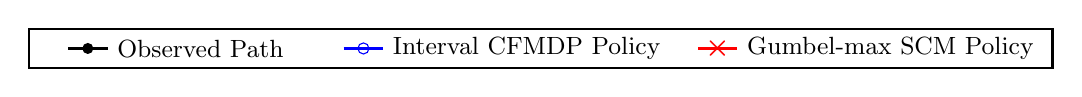
\begin{tikzpicture}[scale=1.0, every node/.style={scale=1.0}]
            \draw[thick, black] (-3, -0.25) rectangle (10, 0.25);
            %
            \draw[black, line width=1pt] (-2.5, 0.0) -- (-2,0.0);
            \fill[black] (-2.25,0.0) circle (2pt); %
            \node[right] at (-2,0.0) {\small Observed Path};
            
            %
            \draw[blue, line width=1pt] (1.0,0.0) -- (1.5,0.0);
            \node[draw=blue, circle, minimum size=4pt, inner sep=0pt] at (1.25,0.0) {}; %
            \node[right] at (1.5,0.0) {\small Interval CFMDP Policy};
            
            %
            \draw[red, line width=1pt] (5.5,0) -- (6,0);
            \node[red] at (5.75,0) {$\boldsymbol{\times}$}; %
            \node[right] at (6,0) {\small Gumbel-max SCM Policy};
        \end{tikzpicture}
    }\\
    %
    \subfigure[\footnotesize Lowest cumulative reward: Interval CFMDP ($312$), Gumbel-max SCM ($312$)]{%
        \resizebox{0.76\columnwidth}{!}{
             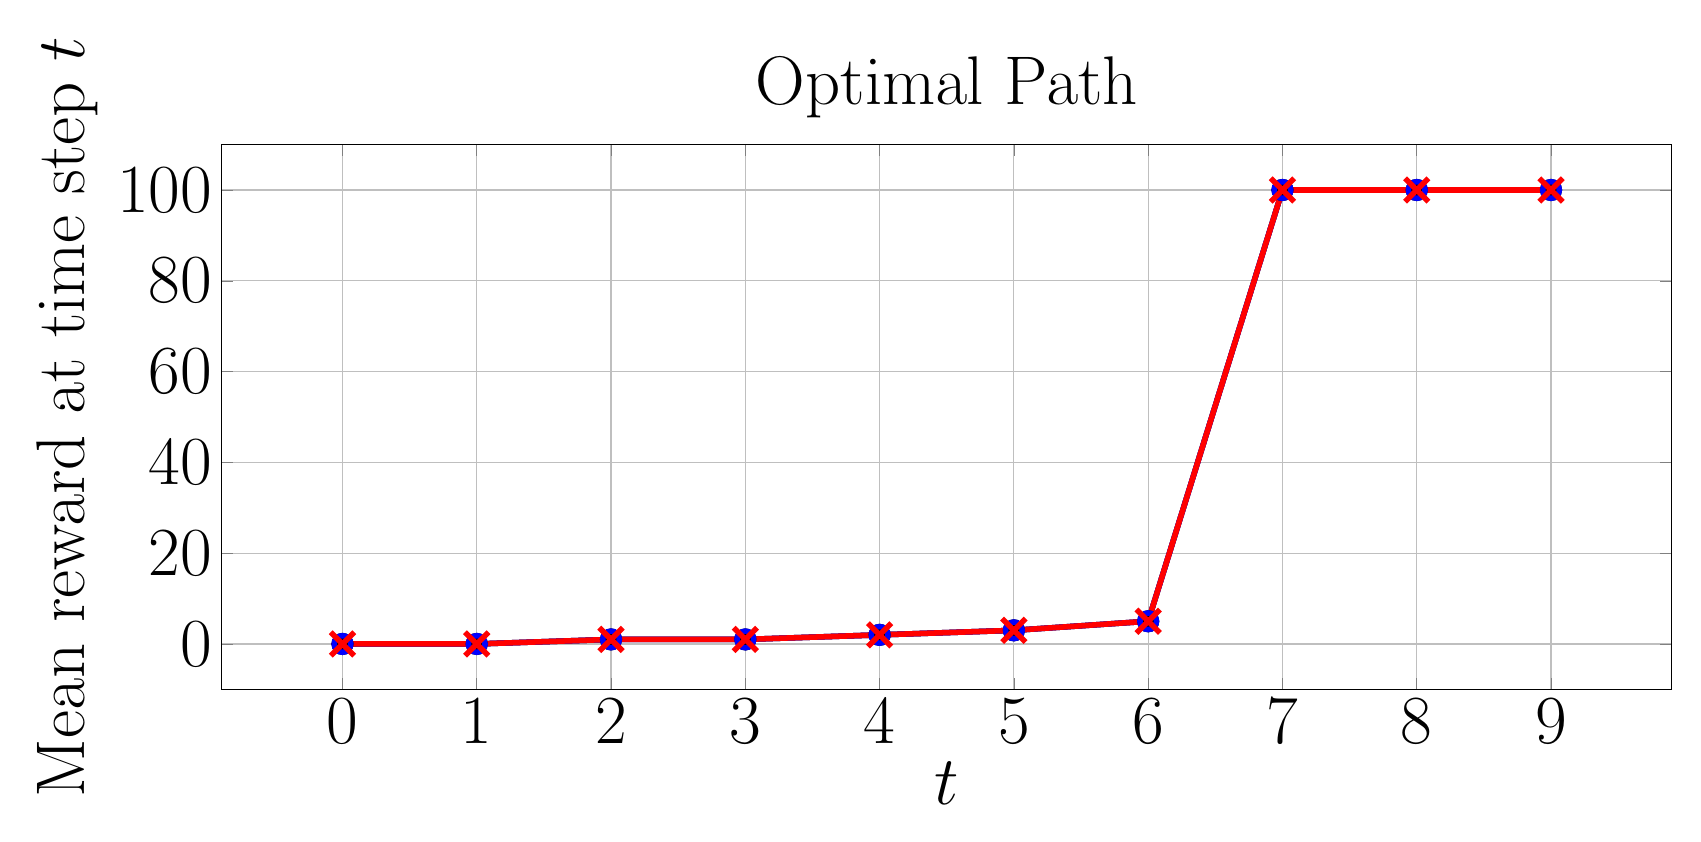
\begin{tikzpicture}
                \begin{axis}[
                    xlabel={$t$},
                    ylabel={Mean reward at time step $t$},
                    title={Optimal Path},
                    grid=both,
                    width=20cm, height=8.5cm,
                    every axis/.style={font=\Huge},
                    %
                ]
                \addplot[
                    color=black, %
                    mark=*, %
                    line width=2pt,
                    mark size=3pt,
                    error bars/.cd,
                    y dir=both, %
                    y explicit, %
                    error bar style={line width=1pt,solid},
                    error mark options={line width=1pt,mark size=4pt,rotate=90}
                ]
                coordinates {
                    (0, 0.0)  +- (0, 0.0)
                    (1, 0.0)  +- (0, 0.0) 
                    (2, 1.0)  +- (0, 0.0) 
                    (3, 1.0)  +- (0, 0.0)
                    (4, 2.0)  +- (0, 0.0)
                    (5, 3.0) +- (0, 0.0)
                    (6, 5.0) +- (0, 0.0)
                    (7, 100.0) +- (0, 0.0)
                    (8, 100.0) +- (0, 0.0)
                    (9, 100.0) +- (0, 0.0)
                };
                %
                \addplot[
                    color=blue, %
                    mark=o, %
                    line width=2pt,
                    mark size=3pt,
                    error bars/.cd,
                    y dir=both, %
                    y explicit, %
                    error bar style={line width=1pt,solid},
                    error mark options={line width=1pt,mark size=4pt,rotate=90}
                ]
                 coordinates {
                    (0, 0.0)  +- (0, 0.0)
                    (1, 0.0)  +- (0, 0.0) 
                    (2, 1.0)  +- (0, 0.0) 
                    (3, 1.0)  +- (0, 0.0)
                    (4, 2.0)  +- (0, 0.0)
                    (5, 3.0) +- (0, 0.0)
                    (6, 5.0) +- (0, 0.0)
                    (7, 100.0) +- (0, 0.0)
                    (8, 100.0) +- (0, 0.0)
                    (9, 100.0) +- (0, 0.0)
                };
                %
                \addplot[
                    color=red, %
                    mark=x, %
                    line width=2pt,
                    mark size=6pt,
                    error bars/.cd,
                    y dir=both, %
                    y explicit, %
                    error bar style={line width=1pt,solid},
                    error mark options={line width=1pt,mark size=4pt,rotate=90}
                ]
                coordinates {
                    (0, 0.0)  +- (0, 0.0)
                    (1, 0.0)  +- (0, 0.0) 
                    (2, 1.0)  +- (0, 0.0) 
                    (3, 1.0)  +- (0, 0.0)
                    (4, 2.0)  +- (0, 0.0)
                    (5, 3.0) +- (0, 0.0)
                    (6, 5.0) +- (0, 0.0)
                    (7, 100.0) +- (0, 0.0)
                    (8, 100.0) +- (0, 0.0)
                    (9, 100.0) +- (0, 0.0)
                };
                \end{axis}
            \end{tikzpicture}
         }
    }
    \hspace{1cm}
    \subfigure[\footnotesize Lowest cumulative reward: Interval CFMDP ($19$), Gumbel-max SCM ($-88$)]{%
         \resizebox{0.76\columnwidth}{!}{
            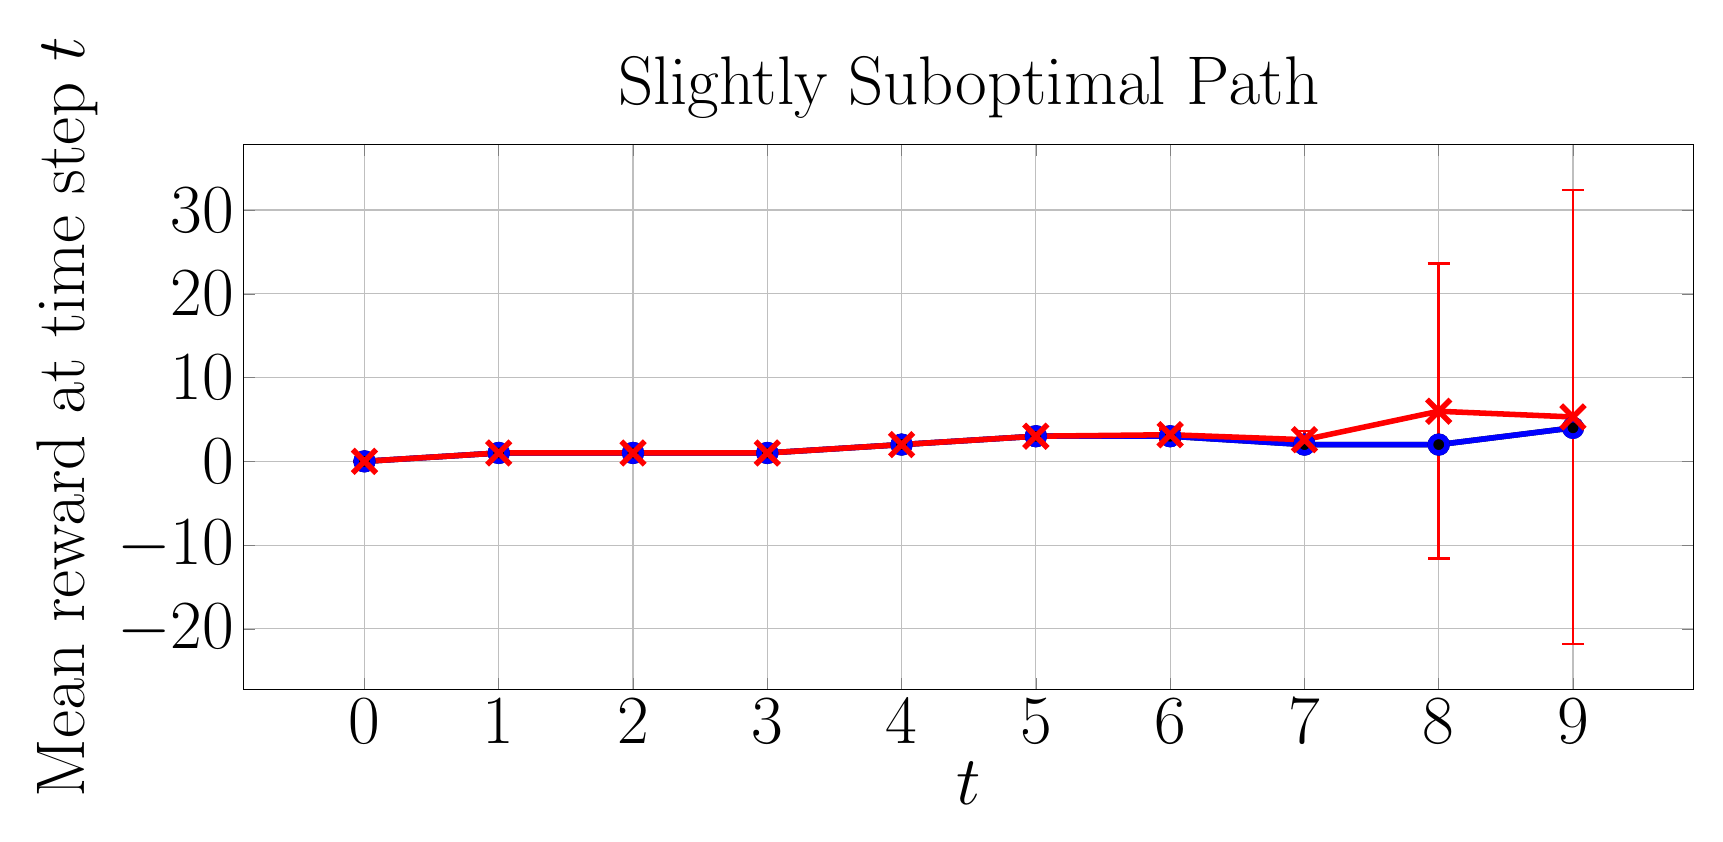
\begin{tikzpicture}
                \begin{axis}[
                    xlabel={$t$},
                    ylabel={Mean reward at time step $t$},
                    title={Slightly Suboptimal Path},
                    grid=both,
                    width=20cm, height=8.5cm,
                    every axis/.style={font=\Huge},
                    %
                ]
                \addplot[
                    color=black, %
                    mark=*, %
                    line width=2pt,
                    mark size=3pt,
                    error bars/.cd,
                    y dir=both, %
                    y explicit, %
                    error bar style={line width=1pt,solid},
                    error mark options={line width=1pt,mark size=4pt,rotate=90}
                ]
              coordinates {
                    (0, 0.0)  +- (0, 0.0)
                    (1, 1.0)  +- (0, 0.0) 
                    (2, 1.0)  +- (0, 0.0) 
                    (3, 1.0)  +- (0, 0.0)
                    (4, 2.0)  +- (0, 0.0)
                    (5, 3.0) +- (0, 0.0)
                    (6, 3.0) +- (0, 0.0)
                    (7, 2.0) +- (0, 0.0)
                    (8, 2.0) +- (0, 0.0)
                    (9, 4.0) +- (0, 0.0)
                };
                %
                \addplot[
                    color=blue, %
                    mark=o, %
                    line width=2pt,
                    mark size=3pt,
                    error bars/.cd,
                    y dir=both, %
                    y explicit, %
                    error bar style={line width=1pt,solid},
                    error mark options={line width=1pt,mark size=4pt,rotate=90}
                ]
              coordinates {
                    (0, 0.0)  +- (0, 0.0)
                    (1, 1.0)  +- (0, 0.0) 
                    (2, 1.0)  +- (0, 0.0) 
                    (3, 1.0)  +- (0, 0.0)
                    (4, 2.0)  +- (0, 0.0)
                    (5, 3.0) +- (0, 0.0)
                    (6, 3.0) +- (0, 0.0)
                    (7, 2.0) +- (0, 0.0)
                    (8, 2.0) +- (0, 0.0)
                    (9, 4.0) +- (0, 0.0)
                };
                %
                \addplot[
                    color=red, %
                    mark=x, %
                    line width=2pt,
                    mark size=6pt,
                    error bars/.cd,
                    y dir=both, %
                    y explicit, %
                    error bar style={line width=1pt,solid},
                    error mark options={line width=1pt,mark size=4pt,rotate=90}
                ]
                coordinates {
                    (0, 0.0)  +- (0, 0.0)
                    (1, 1.0)  +- (0, 0.0) 
                    (2, 1.0)  +- (0, 0.0) 
                    (3, 1.0)  +- (0, 0.0)
                    (4, 2.0)  += (0, 0.0)
                    (5, 3.0)  += (0, 0.0)
                    (6, 3.17847) += (0, 0.62606746) -= (0, 0.62606746)
                    (7, 2.5832885) += (0, 1.04598233) -= (0, 1.04598233)
                    (8, 5.978909) += (0, 17.60137623) -= (0, 17.60137623)
                    (9, 5.297059) += (0, 27.09227512) -= (0, 27.09227512)
                };
                \end{axis}
            \end{tikzpicture}
         }
    }\\[-1.5pt]
    \subfigure[\footnotesize Lowest cumulative reward: Interval CFMDP ($14$), Gumbel-max SCM ($-598$)]{%
         \resizebox{0.76\columnwidth}{!}{
             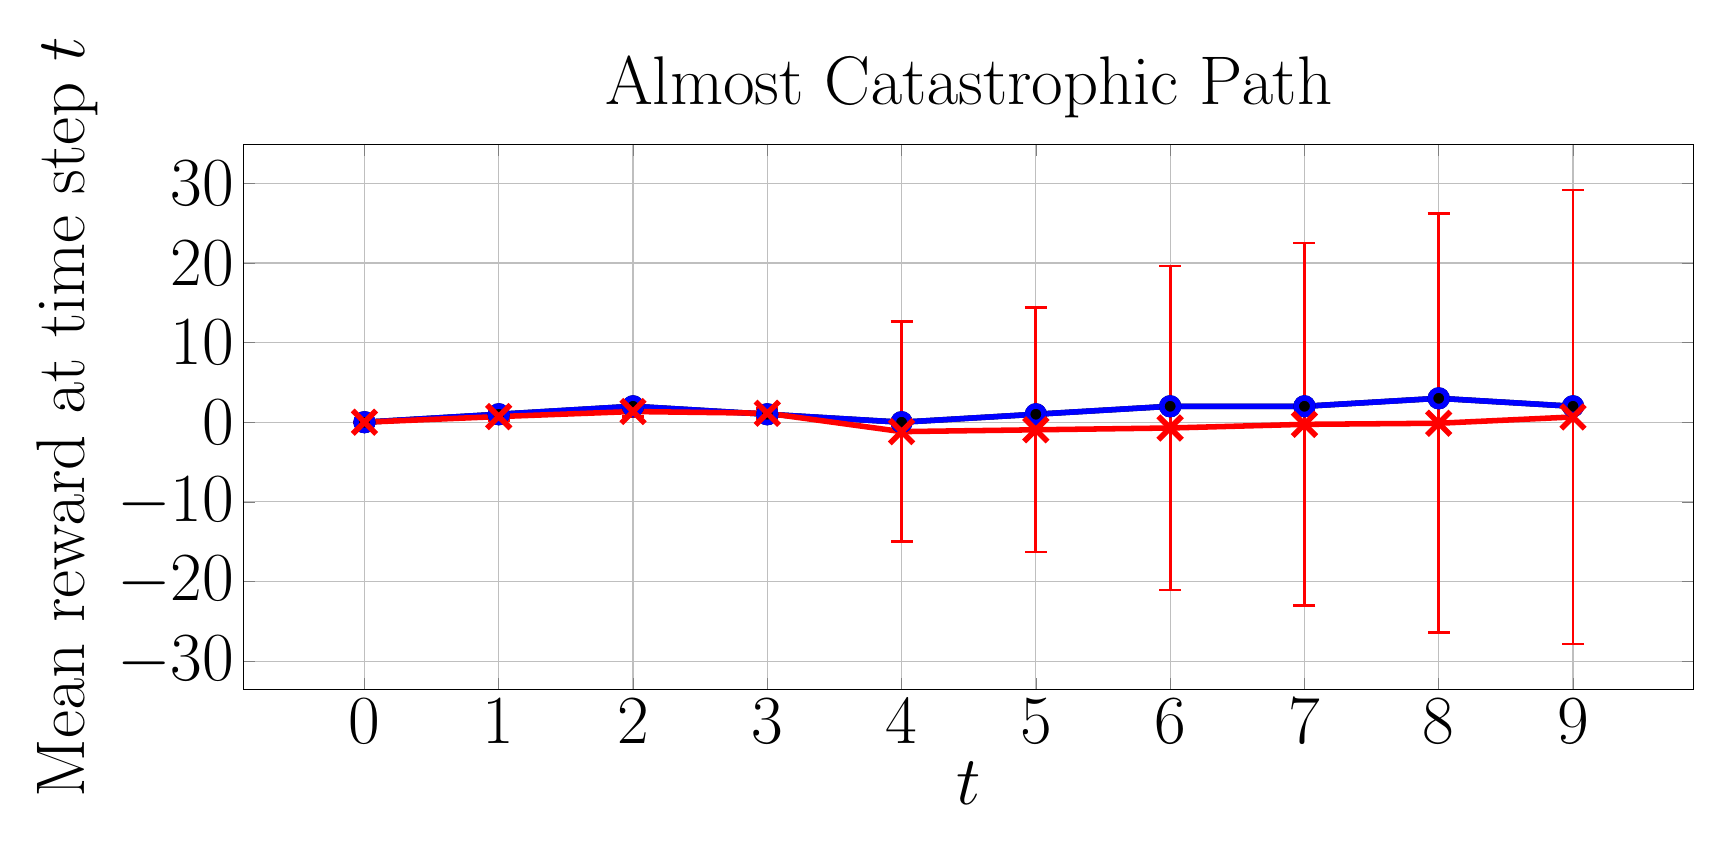
\begin{tikzpicture}
                \begin{axis}[
                    xlabel={$t$},
                    ylabel={Mean reward at time step $t$},
                    title={Almost Catastrophic Path},
                    grid=both,
                    width=20cm, height=8.5cm,
                    every axis/.style={font=\Huge},
                    %
                ]
                \addplot[
                    color=black, %
                    mark=*, %
                    line width=2pt,
                    mark size=3pt,
                    error bars/.cd,
                    y dir=both, %
                    y explicit, %
                    error bar style={line width=1pt,solid},
                    error mark options={line width=1pt,mark size=4pt,rotate=90}
                ]
                coordinates {
                    (0, 0.0)  +- (0, 0.0)
                    (1, 1.0)  +- (0, 0.0) 
                    (2, 2.0)  +- (0, 0.0) 
                    (3, 1.0)  +- (0, 0.0)
                    (4, 0.0)  +- (0, 0.0)
                    (5, 1.0) +- (0, 0.0)
                    (6, 2.0) +- (0, 0.0)
                    (7, 2.0) +- (0, 0.0)
                    (8, 3.0) +- (0, 0.0)
                    (9, 2.0) +- (0, 0.0)
                };
                %
                \addplot[
                    color=blue, %
                    mark=o, %
                    line width=2pt,
                    mark size=3pt,
                    error bars/.cd,
                    y dir=both, %
                    y explicit, %
                    error bar style={line width=1pt,solid},
                    error mark options={line width=1pt,mark size=4pt,rotate=90}
                ]
                coordinates {
                    (0, 0.0)  +- (0, 0.0)
                    (1, 1.0)  +- (0, 0.0) 
                    (2, 2.0)  +- (0, 0.0) 
                    (3, 1.0)  +- (0, 0.0)
                    (4, 0.0)  +- (0, 0.0)
                    (5, 1.0) +- (0, 0.0)
                    (6, 2.0) +- (0, 0.0)
                    (7, 2.0) +- (0, 0.0)
                    (8, 3.0) +- (0, 0.0)
                    (9, 2.0) +- (0, 0.0)
                };
                %
                \addplot[
                    color=red, %
                    mark=x, %
                    line width=2pt,
                    mark size=6pt,
                    error bars/.cd,
                    y dir=both, %
                    y explicit, %
                    error bar style={line width=1pt,solid},
                    error mark options={line width=1pt,mark size=4pt,rotate=90}
                ]
                coordinates {
                    (0, 0.0)  +- (0, 0.0)
                    (1, 0.7065655)  +- (0, 0.4553358) 
                    (2, 1.341673)  +- (0, 0.67091621) 
                    (3, 1.122926)  +- (0, 0.61281824)
                    (4, -1.1821935)  +- (0, 13.82444042)
                    (5, -0.952399)  +- (0, 15.35195457)
                    (6, -0.72672) +- (0, 20.33508414)
                    (7, -0.268983) +- (0, 22.77861454)
                    (8, -0.1310835) +- (0, 26.31013314)
                    (9, 0.65806) +- (0, 28.50670214)
                };
                %
            %
            %
            %
            %
            %
            %
            %
            %
            %
            %
            %
            %
            %
            %
            %
            %
            %
            %
                \end{axis}
            \end{tikzpicture}
         }
    }
    \hspace{1cm}
    \subfigure[\footnotesize Lowest cumulative reward: Interval CFMDP ($-698$), Gumbel-max SCM ($-698$)]{%
         \resizebox{0.76\columnwidth}{!}{
            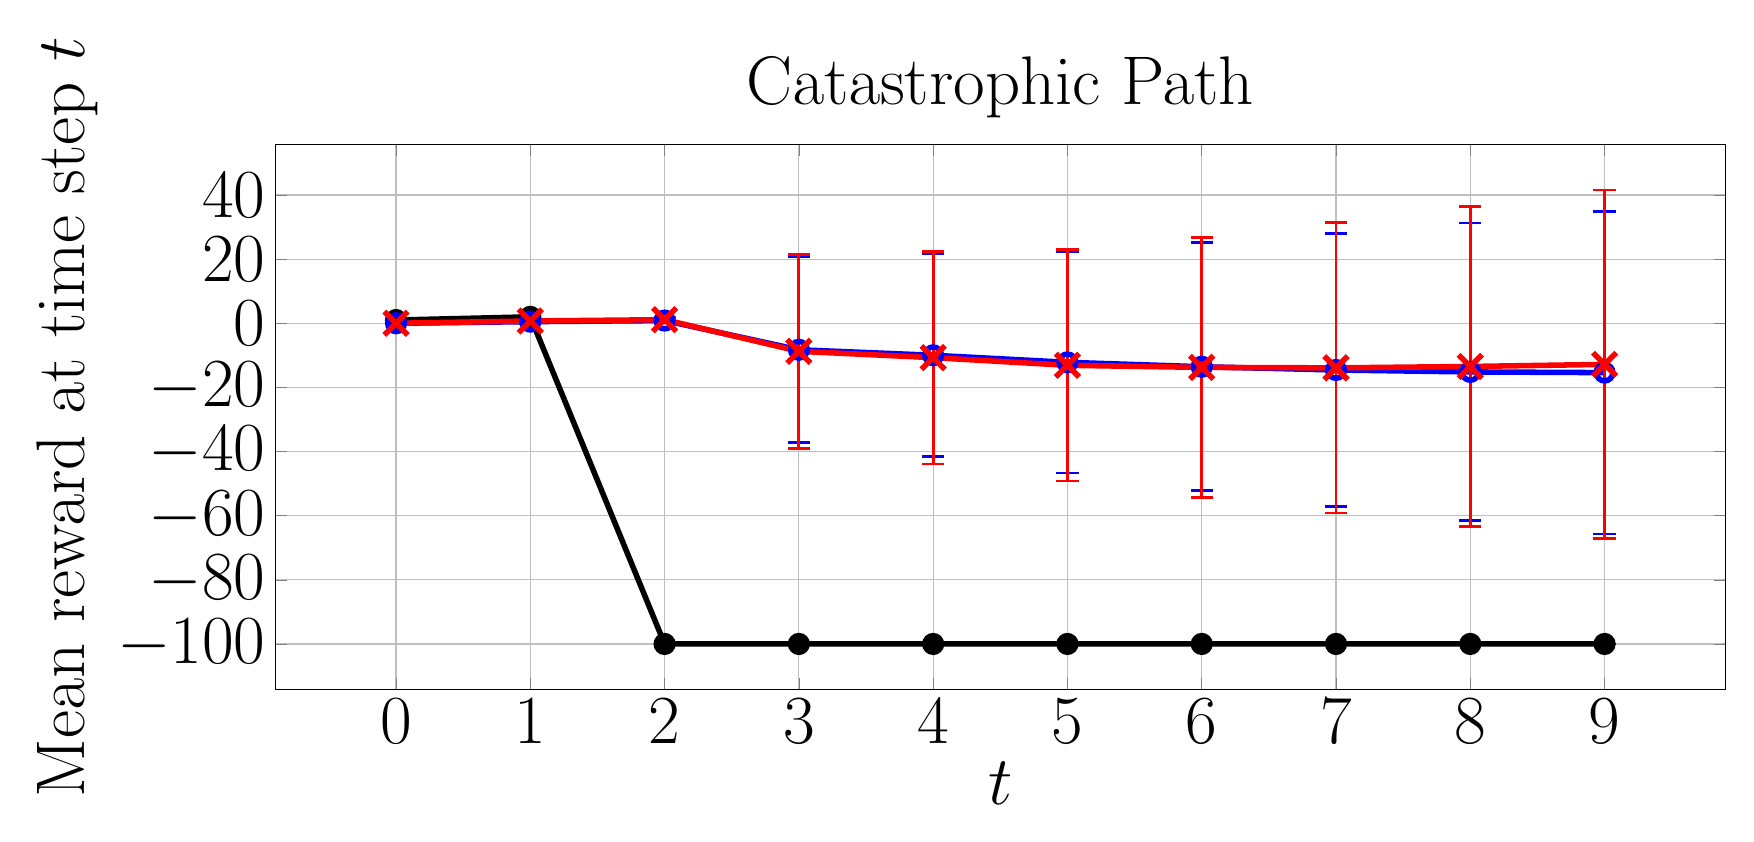
\begin{tikzpicture}
                \begin{axis}[
                    xlabel={$t$},
                    ylabel={Mean reward at time step $t$},
                    title={Catastrophic Path},
                    grid=both,
                    width=20cm, height=8.5cm,
                    every axis/.style={font=\Huge},
                    %
                ]
                \addplot[
                    color=black, %
                    mark=*, %
                    line width=2pt,
                    mark size=3pt,
                    error bars/.cd,
                    y dir=both, %
                    y explicit, %
                    error bar style={line width=1pt,solid},
                    error mark options={line width=1pt,mark size=4pt,rotate=90}
                ]
                coordinates {
                    (0, 1.0)  +- (0, 0.0)
                    (1, 2.0)  +- (0, 0.0) 
                    (2, -100.0)  +- (0, 0.0) 
                    (3, -100.0)  +- (0, 0.0)
                    (4, -100.0)  +- (0, 0.0)
                    (5, -100.0) +- (0, 0.0)
                    (6, -100.0) +- (0, 0.0)
                    (7, -100.0) +- (0, 0.0)
                    (8, -100.0) +- (0, 0.0)
                    (9, -100.0) +- (0, 0.0)
                };
                %
                \addplot[
                    color=blue, %
                    mark=o, %
                    line width=2pt,
                    mark size=3pt,
                    error bars/.cd,
                    y dir=both, %
                    y explicit, %
                    error bar style={line width=1pt,solid},
                    error mark options={line width=1pt,mark size=4pt,rotate=90}
                ]
                coordinates {
                    (0, 0.0)  +- (0, 0.0)
                    (1, 0.504814)  +- (0, 0.49997682) 
                    (2, 0.8439835)  +- (0, 0.76831917) 
                    (3, -8.2709165)  +- (0, 28.93656754)
                    (4, -9.981082)  +- (0, 31.66825363)
                    (5, -12.1776325) +- (0, 34.53463233)
                    (6, -13.556076) +- (0, 38.62845372)
                    (7, -14.574418) +- (0, 42.49603359)
                    (8, -15.1757075) +- (0, 46.41913968)
                    (9, -15.3900395) +- (0, 50.33563368)
                };
                %
                \addplot[
                    color=red, %
                    mark=x, %
                    line width=2pt,
                    mark size=6pt,
                    error bars/.cd,
                    y dir=both, %
                    y explicit, %
                    error bar style={line width=1pt,solid},
                    error mark options={line width=1pt,mark size=4pt,rotate=90}
                ]
                coordinates {
                    (0, 0.0)  +- (0, 0.0)
                    (1, 0.701873)  +- (0, 0.45743556) 
                    (2, 1.1227805)  +- (0, 0.73433129) 
                    (3, -8.7503255)  +- (0, 30.30257976)
                    (4, -10.722092)  +- (0, 33.17618589)
                    (5, -13.10721)  +- (0, 36.0648089)
                    (6, -13.7631645) +- (0, 40.56553451)
                    (7, -13.909043) +- (0, 45.23829402)
                    (8, -13.472517) +- (0, 49.96270296)
                    (9, -12.8278835) +- (0, 54.38618735)
                };
                %
            %
            %
            %
            %
            %
            %
            %
            %
            %
            %
            %
            %
            %
            %
            %
            %
            %
            %
                \end{axis}
            \end{tikzpicture}
         }
    }
    \caption{Average instant reward of CF paths induced by policies on GridWorld $p=0.4$.}
    \label{fig: reward p=0.4}
\end{figure*}

\subsection{Experimental Setup}
To compare policy performance, we measure the average rewards of counterfactual paths induced by our policy and the Gumbel-max policy by uniformly sampling $200$ counterfactual MDPs from the ICFMDP and generating $10,000$ counterfactual paths over each sampled CFMDP. \jl{Since the interval CFMDP depends on the observed path, we select $4$  paths of varying optimality to evaluate how the observed path impacts the performance of both policies: an optimal path, a slightly suboptimal path that could reach the optimal reward with a few changes, a catastrophic path that enters a catastrophic, terminal state with low reward, and an almost catastrophic path that was close to entering a catastrophic state.} When measuring the average probability bound widths and execution time needed to generate the ICFMDPs, we averaged over $20$ randomly generated observed paths
\footnote{Further training details are provided in Appendix \ref{app: training details}, and the code is provided at \href{https://github.com/ddv-lab/robust-cf-inference-in-MDPs}{https://github.com/ddv-lab/robust-cf-inference-in-MDPs}
%
%
.}.

\subsection{GridWorld}
\jl{The GridWorld MDP is a $4 \times 4$ grid where an agent must navigate from the top-left corner to the goal state in the bottom-right corner, avoiding a dangerous terminal state in the centre. At each time step, the agent can move up, down, left, or right, but there is a small probability (controlled by hyper-parameter $p$) of moving in an unintended direction. As the agent nears the goal, the reward for each state increases, culminating in a reward of $+100$ for reaching the goal. Entering the dangerous state results in a penalty of $-100$. We use two versions of GridWorld: a less stochastic version with $p=0.9$ (i.e., $90$\% chance of moving in the chosen direction) and a more stochastic version with $p=0.4$.}

\paragraph{GridWorld ($p=0.9$)}
When $p=0.9$, the counterfactual probability bounds are typically narrow (see Table \ref{tab:nonzero_probs} for average measurements). Consequently, as shown in Figure \ref{fig: reward p=0.9}, both policies are nearly identical and perform similarly well across the optimal, slightly suboptimal, and catastrophic paths.
%
However, for the almost catastrophic path, the interval CFMDP path is more conservative and follows the observed path more closely (as this is where the probability bounds are narrowest), which typically requires one additional step to reach the goal state than the Gumbel-max SCM policy.
%

\paragraph{GridWorld ($p=0.4$)}
\jl{When $p=0.4$, the GridWorld environment becomes more uncertain, increasing the risk of entering the dangerous state even if correct actions are chosen. Thus, as shown in Figure \ref{fig: reward p=0.4}, the interval CFMDP policy adopts a more conservative approach, avoiding deviation from the observed policy if it cannot guarantee higher counterfactual rewards (see the slightly suboptimal and almost catastrophic paths), whereas the Gumbel-max SCM is inconsistent: it can yield higher rewards, but also much lower rewards, reflected in the wide error bars.} For the catastrophic path, both policies must deviate from the observed path to achieve a higher reward and, in this case, perform similarly.
%
%
%
%
\subsection{Sepsis}
The Sepsis MDP \citep{oberst2019counterfactual} simulates trajectories of Sepsis patients. Each state consists of four vital signs (heart rate, blood pressure, oxygen concentration, and glucose levels), categorised as low, normal, or high.
and three treatments that can be toggled on/off at each time step (8 actions in total). Unlike \citet{oberst2019counterfactual}, we scale rewards based on the number of out-of-range vital signs, between $-1000$ (patient dies) and $1000$ (patient discharged). \jl{Like the GridWorld $p=0.4$ experiment, the Sepsis MDP is highly uncertain, as many states are equally likely to lead to optimal and poor outcomes. Thus, as shown in Figure \ref{fig: reward sepsis}, both policies follow the observed optimal and almost catastrophic paths to guarantee rewards are no worse than the observation.} However, improving the catastrophic path requires deviating from the observation. Here, the Gumbel-max SCM policy, on average, performs better than the interval CFMDP policy. But, since both policies have lower bounds clipped at $-1000$, neither policy reliably improves over the observation. In contrast, for the slightly suboptimal path, the interval CFMDP policy performs significantly better, shown by its higher lower bounds. 
Moreover, in these two cases, the worst-case counterfactual path generated by the interval CFMDP policy is better than that of the Gumbel-max SCM policy,
indicating its greater robustness.
%
\begin{figure*}
    \centering
     \resizebox{0.6\textwidth}{!}{
        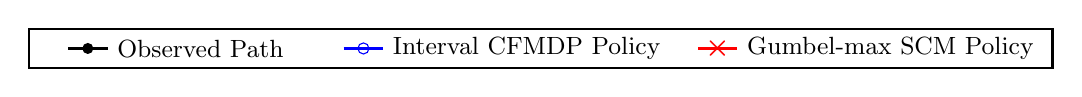
\begin{tikzpicture}[scale=1.0, every node/.style={scale=1.0}]
            \draw[thick, black] (-3, -0.25) rectangle (10, 0.25);
            %
            \draw[black, line width=1pt] (-2.5, 0.0) -- (-2,0.0);
            \fill[black] (-2.25,0.0) circle (2pt); %
            \node[right] at (-2,0.0) {\small Observed Path};
            
            %
            \draw[blue, line width=1pt] (1.0,0.0) -- (1.5,0.0);
            \node[draw=blue, circle, minimum size=4pt, inner sep=0pt] at (1.25,0.0) {}; %
            \node[right] at (1.5,0.0) {\small Interval CFMDP Policy};
            
            %
            \draw[red, line width=1pt] (5.5,0) -- (6,0);
            \node[red] at (5.75,0) {$\boldsymbol{\times}$}; %
            \node[right] at (6,0) {\small Gumbel-max SCM Policy};
        \end{tikzpicture}
    }\\
    \subfigure[\footnotesize Lowest cumulative reward: Interval CFMDP ($8000$), Gumbel-max SCM ($8000$)]{%
         \resizebox{0.76\columnwidth}{!}{
             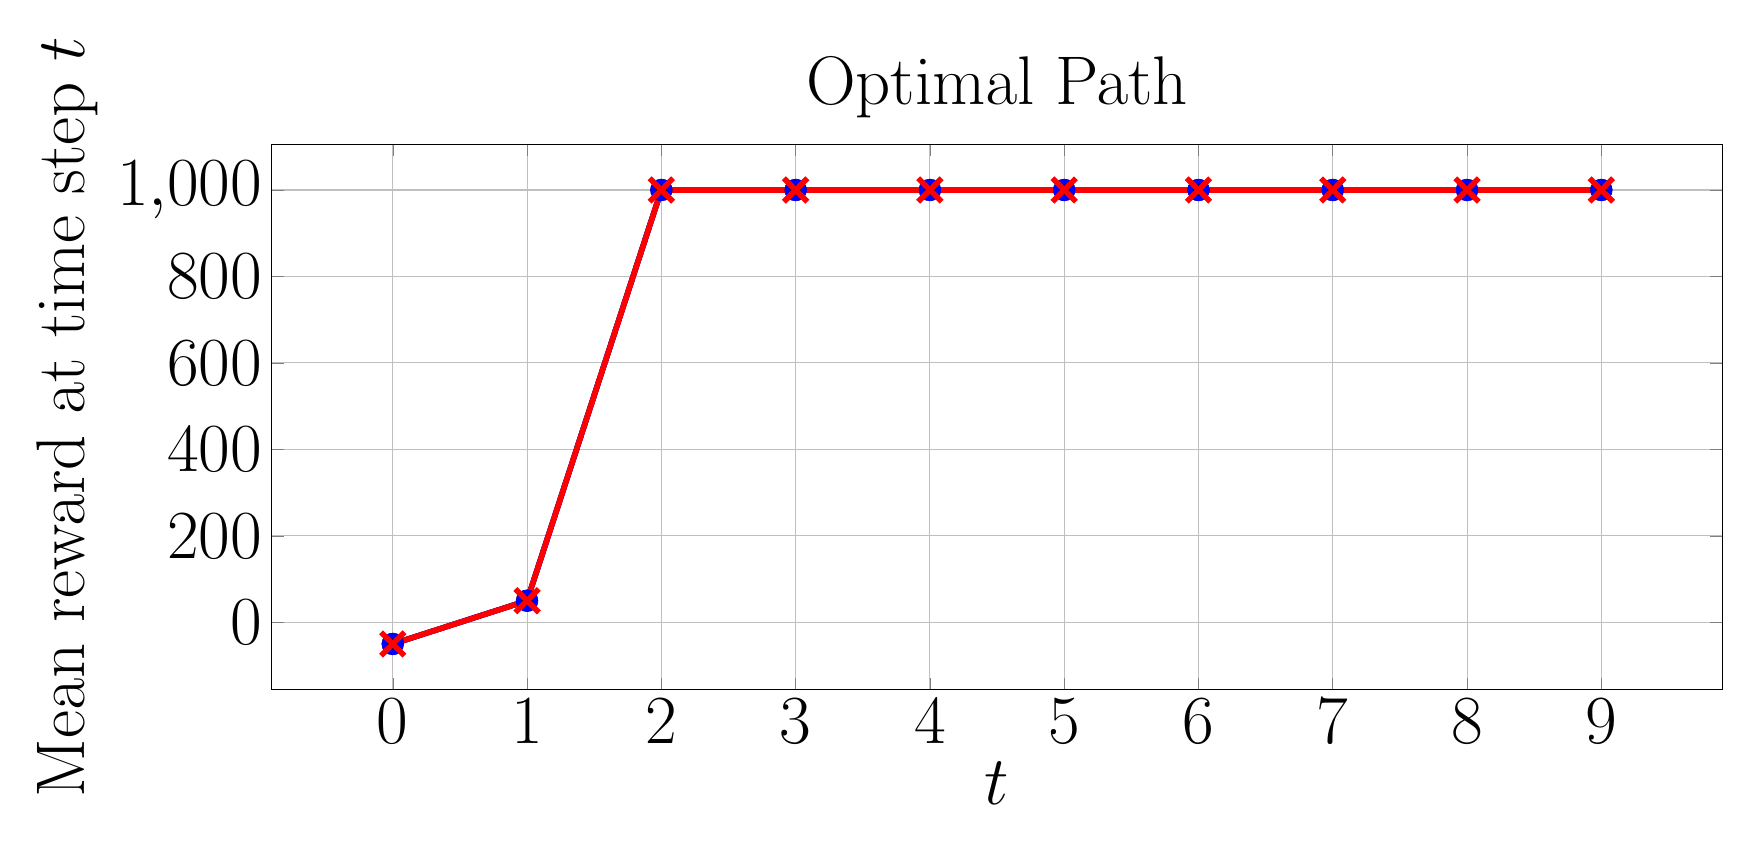
\begin{tikzpicture}
                \begin{axis}[
                    xlabel={$t$},
                    ylabel={Mean reward at time step $t$},
                    title={Optimal Path},
                    grid=both,
                    width=20cm, height=8.5cm,
                    every axis/.style={font=\Huge},
                    %
                ]
                \addplot[
                    color=black, %
                    mark=*, %
                    line width=2pt,
                    mark size=3pt,
                ]
                coordinates {
                    (0, -50.0)
                    (1, 50.0)
                    (2, 1000.0)
                    (3, 1000.0)
                    (4, 1000.0)
                    (5, 1000.0)
                    (6, 1000.0)
                    (7, 1000.0)
                    (8, 1000.0)
                    (9, 1000.0)
                };
                %
                \addplot[
                    color=blue, %
                    mark=o, %
                    line width=2pt,
                    mark size=3pt,
                    error bars/.cd,
                    y dir=both, %
                    y explicit, %
                    error bar style={line width=1pt,solid},
                    error mark options={line width=1pt,mark size=4pt,rotate=90}
                ]
                coordinates {
                    (0, -50.0)  +- (0, 0.0)
                    (1, 50.0)  +- (0, 0.0) 
                    (2, 1000.0)  +- (0, 0.0) 
                    (3, 1000.0)  +- (0, 0.0)
                    (4, 1000.0)  +- (0, 0.0)
                    (5, 1000.0) +- (0, 0.0)
                    (6, 1000.0) +- (0, 0.0)
                    (7, 1000.0) +- (0, 0.0)
                    (8, 1000.0) +- (0, 0.0)
                    (9, 1000.0) +- (0, 0.0)
                };
                %
                \addplot[
                    color=red, %
                    mark=x, %
                    line width=2pt,
                    mark size=6pt,
                    error bars/.cd,
                    y dir=both, %
                    y explicit, %
                    error bar style={line width=1pt,solid},
                    error mark options={line width=1pt,mark size=4pt,rotate=90}
                ]
                coordinates {
                    (0, -50.0)  +- (0, 0.0)
                    (1, 50.0)  +- (0, 0.0) 
                    (2, 1000.0)  +- (0, 0.0) 
                    (3, 1000.0)  +- (0, 0.0)
                    (4, 1000.0)  +- (0, 0.0)
                    (5, 1000.0) +- (0, 0.0)
                    (6, 1000.0) +- (0, 0.0)
                    (7, 1000.0) +- (0, 0.0)
                    (8, 1000.0) +- (0, 0.0)
                    (9, 1000.0) +- (0, 0.0)
                };
                %
                \end{axis}
            \end{tikzpicture}
         }
    }
    \hspace{1cm}
    \subfigure[\footnotesize Lowest cumulative reward: Interval CFMDP ($-5980$), Gumbel-max SCM ($-8000$)]{%
         \resizebox{0.76\columnwidth}{!}{
            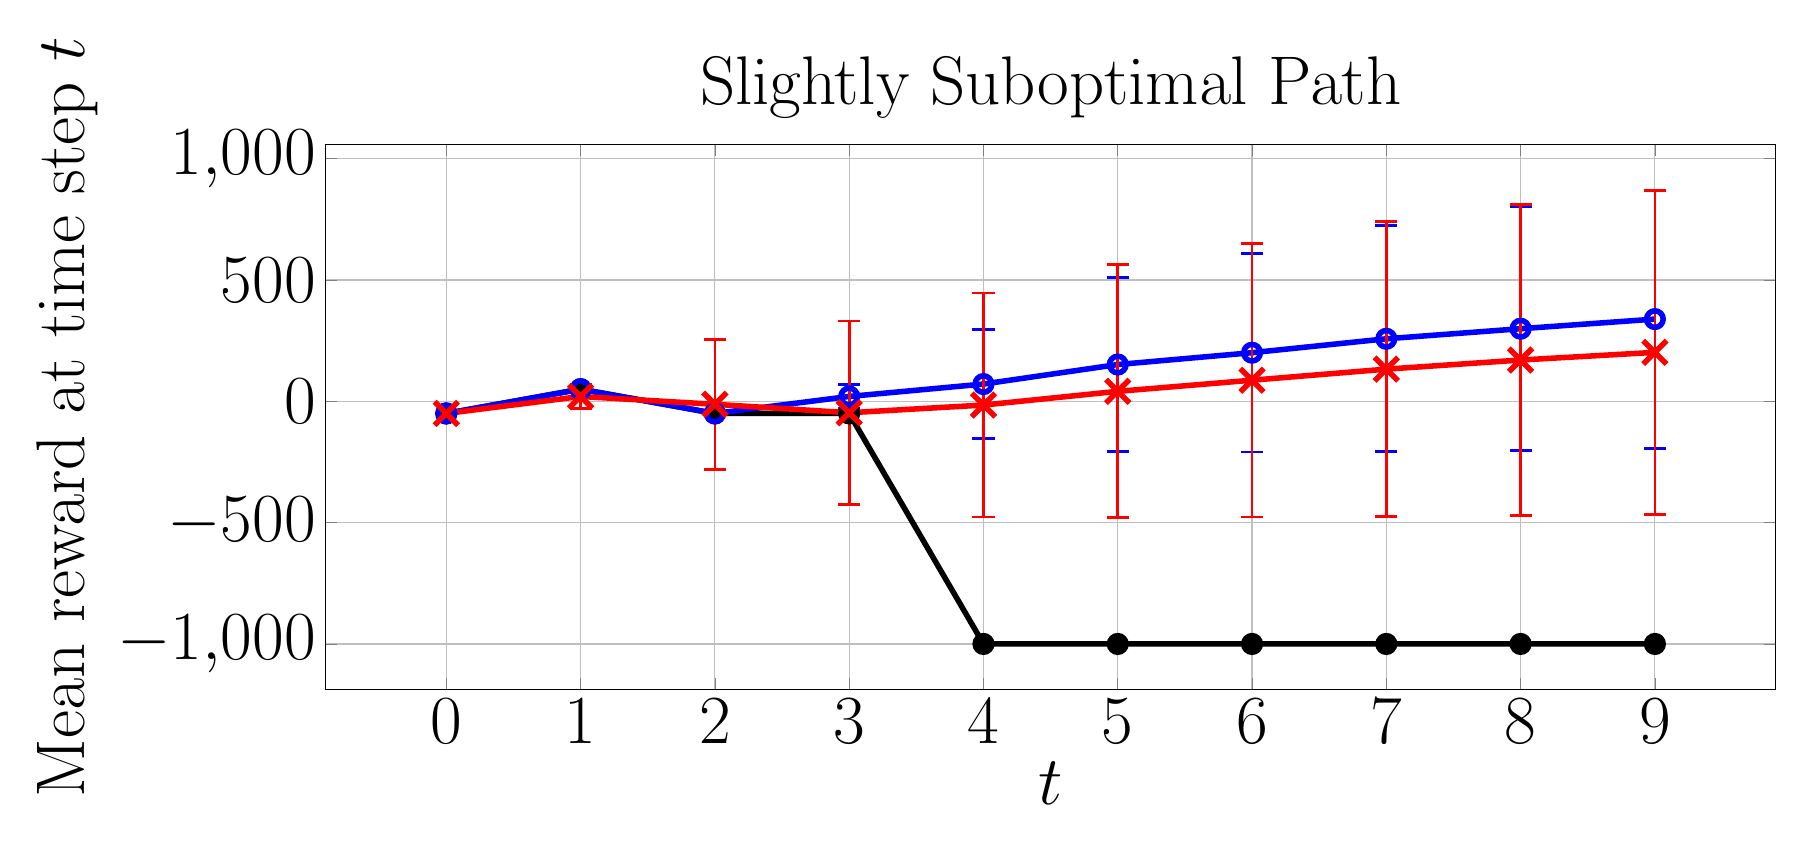
\begin{tikzpicture}
                \begin{axis}[
                    xlabel={$t$},
                    ylabel={Mean reward at time step $t$},
                    title={Slightly Suboptimal Path},
                    grid=both,
                    width=20cm, height=8.5cm,
                    every axis/.style={font=\Huge},
                    %
                ]
               \addplot[
                    color=black, %
                    mark=*, %
                    line width=2pt,
                    mark size=3pt,
                ]
                coordinates {
                    (0, -50.0)
                    (1, 50.0)
                    (2, -50.0)
                    (3, -50.0)
                    (4, -1000.0)
                    (5, -1000.0)
                    (6, -1000.0)
                    (7, -1000.0)
                    (8, -1000.0)
                    (9, -1000.0)
                };
                %
                \addplot[
                    color=blue, %
                    mark=o, %
                    line width=2pt,
                    mark size=3pt,
                    error bars/.cd,
                    y dir=both, %
                    y explicit, %
                    error bar style={line width=1pt,solid},
                    error mark options={line width=1pt,mark size=4pt,rotate=90}
                ]
                coordinates {
                    (0, -50.0)  +- (0, 0.0)
                    (1, 50.0)  +- (0, 0.0) 
                    (2, -50.0)  +- (0, 0.0) 
                    (3, 20.0631)  +- (0, 49.97539413)
                    (4, 71.206585)  +- (0, 226.02033693)
                    (5, 151.60797) +- (0, 359.23292559)
                    (6, 200.40593) +- (0, 408.86185176)
                    (7, 257.77948) +- (0, 466.10372804)
                    (8, 299.237465) +- (0, 501.82579506)
                    (9, 338.9129) +- (0, 532.06124996)
                };
                %
                \addplot[
                    color=red, %
                    mark=x, %
                    line width=2pt,
                    mark size=6pt,
                    error bars/.cd,
                    y dir=both, %
                    y explicit, %
                    error bar style={line width=1pt,solid},
                    error mark options={line width=1pt,mark size=4pt,rotate=90}
                ]
                coordinates {
                    (0, -50.0)  +- (0, 0.0)
                    (1, 20.00736)  +- (0, 49.99786741) 
                    (2, -12.282865)  +- (0, 267.598755) 
                    (3, -47.125995)  +- (0, 378.41755832)
                    (4, -15.381965)  +- (0, 461.77616558)
                    (5, 41.15459) +- (0, 521.53189262)
                    (6, 87.01595) +- (0, 564.22243126 )
                    (7, 132.62376) +- (0, 607.31338037)
                    (8, 170.168145) +- (0, 641.48013693)
                    (9, 201.813135) +- (0, 667.29441777)
                };
                %
                %
                %
                %
                %
                %
                %
                %
                %
                %
                %
                %
                %
                %
                %
                %
                %
                %
                %
                \end{axis}
            \end{tikzpicture}
         }
    }\\[-1.5pt]
    \subfigure[\footnotesize Lowest cumulative reward: Interval CFMDP ($100$), Gumbel-max SCM ($100$)]{%
         \resizebox{0.76\columnwidth}{!}{
             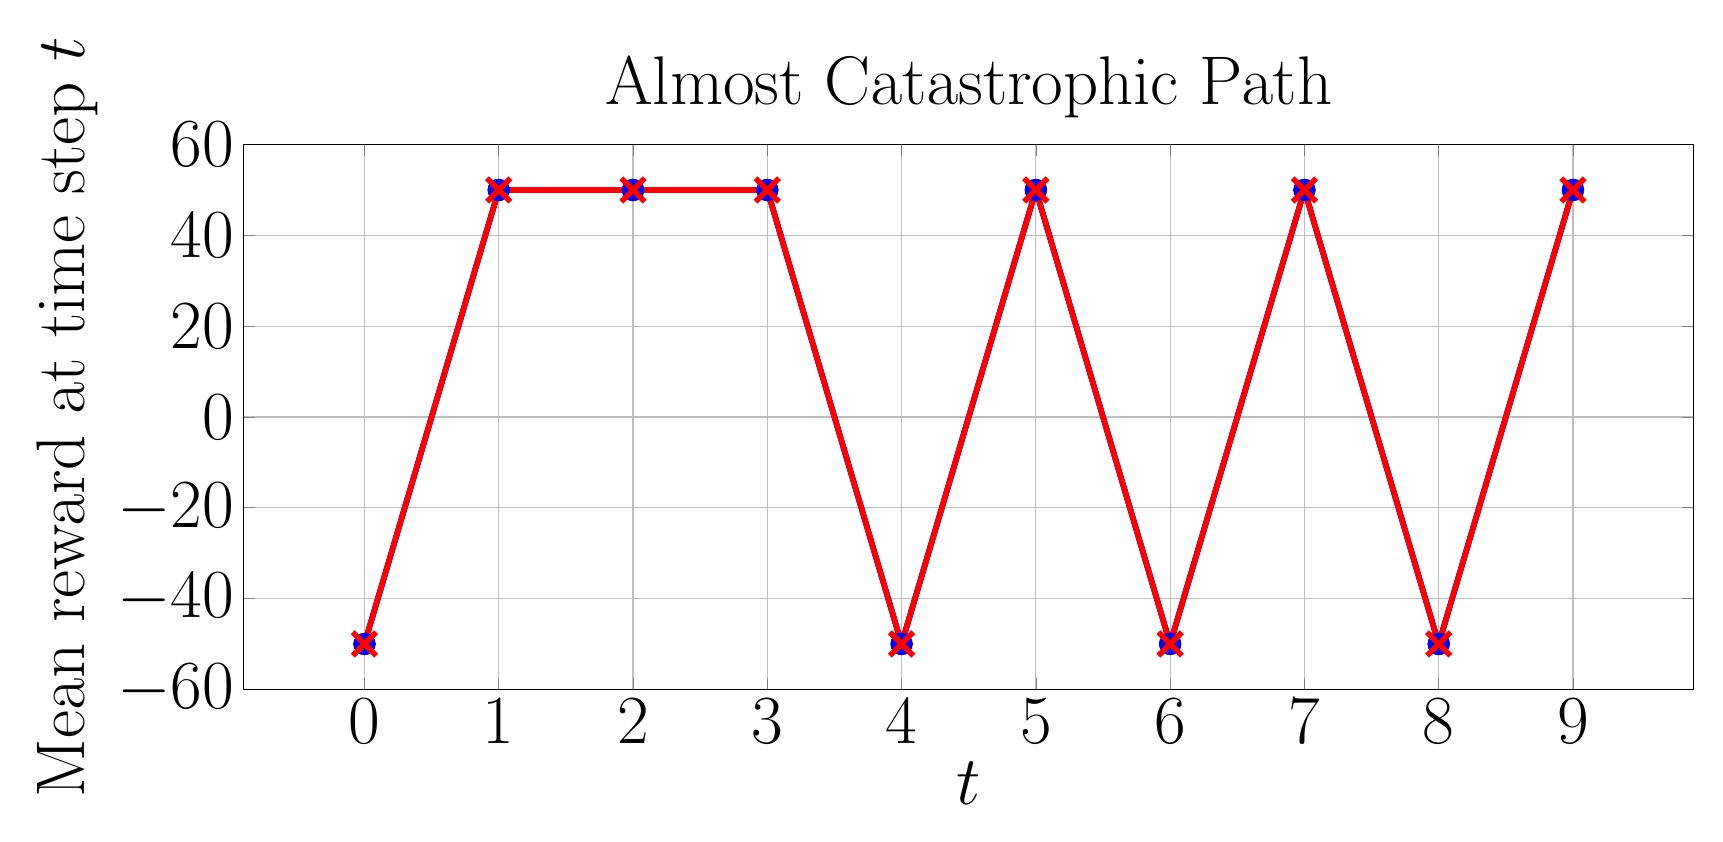
\begin{tikzpicture}
                \begin{axis}[
                    xlabel={$t$},
                    ylabel={Mean reward at time step $t$},
                    title={Almost Catastrophic Path},
                    grid=both,
                    every axis/.style={font=\Huge},
                    width=20cm, height=8.5cm,
                    %
                ]
               \addplot[
                    color=black, %
                    mark=*, %
                    line width=2pt,
                    mark size=3pt,
                ]
                coordinates {
                    (0, -50.0)
                    (1, 50.0)
                    (2, 50.0)
                    (3, 50.0)
                    (4, -50.0)
                    (5, 50.0)
                    (6, -50.0)
                    (7, 50.0)
                    (8, -50.0)
                    (9, 50.0)
                };
                %
                %
                \addplot[
                    color=blue, %
                    mark=o, %
                    line width=2pt,
                    mark size=3pt,
                    error bars/.cd,
                    y dir=both, %
                    y explicit, %
                    error bar style={line width=1pt,solid},
                    error mark options={line width=1pt,mark size=4pt,rotate=90}
                ]
                coordinates {
                    (0, -50.0)  +- (0, 0.0)
                    (1, 50.0)  +- (0, 0.0) 
                    (2, 50.0)  +- (0, 0.0) 
                    (3, 50.0)  +- (0, 0.0)
                    (4, -50.0)  +- (0, 0.0)
                    (5, 50.0) +- (0, 0.0)
                    (6, -50.0) +- (0, 0.0)
                    (7, 50.0) +- (0, 0.0)
                    (8, -50.0) +- (0, 0.0)
                    (9, 50.0) +- (0, 0.0)
                };
                %
                \addplot[
                    color=red, %
                    mark=x, %
                    line width=2pt,
                    mark size=6pt,
                    error bars/.cd,
                    y dir=both, %
                    y explicit, %
                    error bar style={line width=1pt,solid},
                    error mark options={line width=1pt,mark size=4pt,rotate=90}
                ]
                coordinates {
                    (0, -50.0)  +- (0, 0.0)
                    (1, 50.0)  +- (0, 0.0) 
                    (2, 50.0)  +- (0, 0.0) 
                    (3, 50.0)  +- (0, 0.0)
                    (4, -50.0)  +- (0, 0.0)
                    (5, 50.0) +- (0, 0.0)
                    (6, -50.0) +- (0, 0.0)
                    (7, 50.0) +- (0, 0.0)
                    (8, -50.0) +- (0, 0.0)
                    (9, 50.0) +- (0, 0.0)
                };
                %
                %
                %
                %
                %
                %
                %
                %
                %
                %
                %
                %
                %
                %
                %
                %
                %
                %
                %
                \end{axis}
            \end{tikzpicture}
         }
    }
    \hspace{1cm}
    \subfigure[\footnotesize Lowest cumulative reward: Interval CFMDP ($-7150$), Gumbel-max SCM ($-9050$)]{%
         \resizebox{0.76\columnwidth}{!}{
            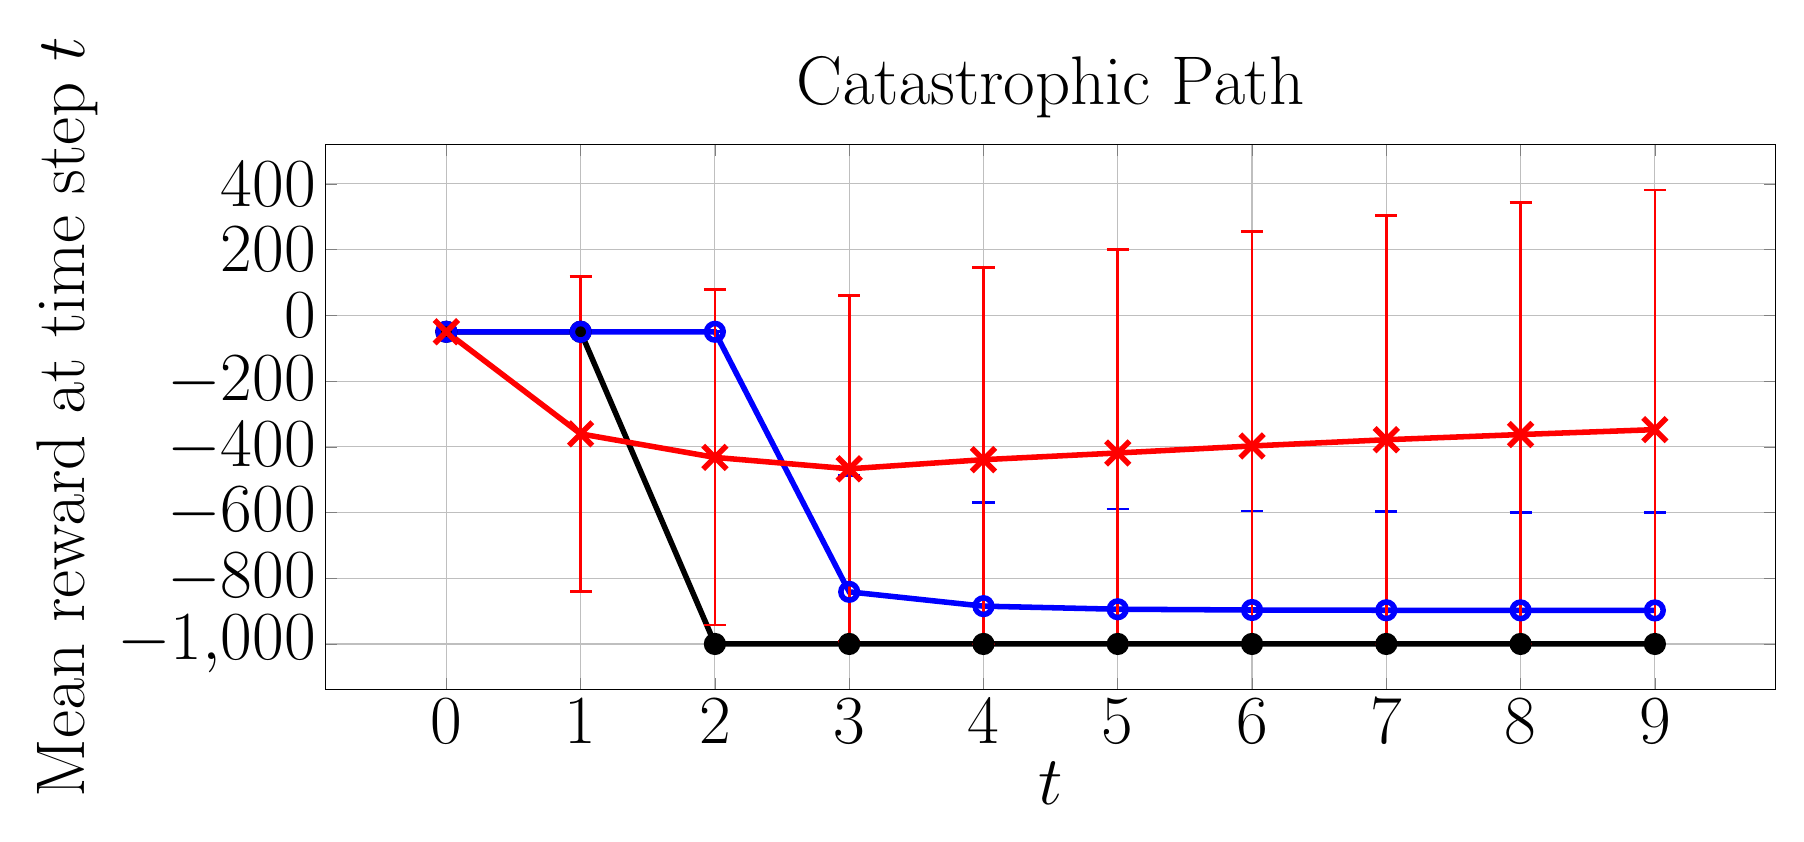
\begin{tikzpicture}
                \begin{axis}[
                    xlabel={$t$},
                    ylabel={Mean reward at time step $t$},
                    title={Catastrophic Path},
                    grid=both,
                    width=20cm, height=8.5cm,
                    every axis/.style={font=\Huge},
                    %
                ]
               \addplot[
                    color=black, %
                    mark=*, %
                    line width=2pt,
                    mark size=3pt,
                ]
                coordinates {
                    (0, -50.0)
                    (1, -50.0)
                    (2, -1000.0)
                    (3, -1000.0)
                    (4, -1000.0)
                    (5, -1000.0)
                    (6, -1000.0)
                    (7, -1000.0)
                    (8, -1000.0)
                    (9, -1000.0)
                };
                %
                %
                \addplot[
                    color=blue, %
                    mark=o, %
                    line width=2pt,
                    mark size=3pt,
                    error bars/.cd,
                    y dir=both, %
                    y explicit, %
                    error bar style={line width=1pt,solid},
                    error mark options={line width=1pt,mark size=4pt,rotate=90}
                ]
                coordinates {
                    (0, -50.0)  +- (0, 0.0)
                    (1, -50.0)  +- (0, 0.0) 
                    (2, -50.0)  +- (0, 0.0) 
                    (3, -841.440725)  += (0, 354.24605512) -= (0, 158.559275)
                    (4, -884.98225)  += (0, 315.37519669) -= (0, 115.01775)
                    (5, -894.330425) += (0, 304.88572805) -= (0, 105.669575)
                    (6, -896.696175) += (0, 301.19954514) -= (0, 103.303825)
                    (7, -897.4635) += (0, 299.61791279) -= (0, 102.5365)
                    (8, -897.77595) += (0, 298.80392585) -= (0, 102.22405)
                    (9, -897.942975) += (0, 298.32920557) -= (0, 102.057025)
                };
                %
                \addplot[
                    color=red, %
                    mark=x, %
                    line width=2pt,
                    mark size=6pt,
                    error bars/.cd,
                    y dir=both, %
                    y explicit, %
                    error bar style={line width=1pt,solid},
                    error mark options={line width=1pt,mark size=4pt,rotate=90}
                ]
            coordinates {
                    (0, -50.0)  +- (0, 0.0)
                    (1, -360.675265)  +- (0, 479.39812699) 
                    (2, -432.27629)  +- (0, 510.38620897) 
                    (3, -467.029545)  += (0, 526.36009628) -= (0, 526.36009628)
                    (4, -439.17429)  += (0, 583.96638919) -= (0, 560.82571)
                    (5, -418.82704) += (0, 618.43027478) -= (0, 581.17296)
                    (6, -397.464895) += (0, 652.67322574) -= (0, 602.535105)
                    (7, -378.49052) += (0, 682.85407033) -= (0, 621.50948)
                    (8, -362.654195) += (0, 707.01412023) -= (0, 637.345805)
                    (9, -347.737935) += (0, 729.29076479) -= (0, 652.262065)
                };
                %
                %
                %
                %
                %
                %
                %
                %
                %
                %
                %
                %
                %
                %
                %
                %
                %
                %
                %
                \end{axis}
            \end{tikzpicture}
         }
    }
    \caption{Average instant reward of CF paths induced by policies on Sepsis.}
    \label{fig: reward sepsis}
\end{figure*}

%
%
%
\subsection{Interval CFMDP Bounds}
%
%
Table \ref{tab:nonzero_probs} presents the mean counterfactual probability bound widths (excluding transitions where the upper bound is $0$) for each MDP, averaged over 20 observed paths. We compare the bounds under counterfactual stability (CS) and monotonicity (M) assumptions, CS alone, and no assumptions. This shows that the assumptions marginally reduce the bound widths, indicating the assumptions tighten the bounds without excluding too many causal models, as intended.
\renewcommand{\arraystretch}{1}

\begin{table}
\centering
\caption{Mean width of counterfactual probability bounds}
\resizebox{0.8\columnwidth}{!}{%
\begin{tabular}{|c|c|c|c|}
\hline
\multirow{2}{*}{\textbf{Environment}} & \multicolumn{3}{c|}{\textbf{Assumptions}} \\ \cline{2-4}
 & \textbf{CS + M} & \textbf{CS} & \textbf{None\tablefootnote{\jl{Equivalent to \citet{li2024probabilities}'s bounds (see Section \ref{sec: equivalence with Li}).}}} \\ \hline
\textbf{GridWorld} ($p=0.9$) & 0.0817 & 0.0977 & 0.100 \\ \hline
\textbf{GridWorld} ($p=0.4$) & 0.552  & 0.638  & 0.646 \\ \hline
\textbf{Sepsis} & 0.138 & 0.140 & 0.140 \\ \hline
\end{tabular}
}
\label{tab:nonzero_probs}
\end{table}


\subsection{Execution Times}
Table \ref{tab: times} compares the average time needed to generate the interval CFMDP vs.\ the Gumbel-max SCM CFMDP for 20 observations.
The GridWorld algorithms were run single-threaded, while the Sepsis experiments were run in parallel.
Generating the interval CFMDP is significantly faster as it uses exact analytical bounds, whereas the Gumbel-max CFMDP requires sampling from the Gumbel distribution to estimate counterfactual transition probabilities. \jl{Since constructing the counterfactual MDP models is the main bottleneck in both approaches, ours is more efficient overall and suitable for larger MDPs.}
\begin{table}
\centering
\caption{Mean execution time to generate CFMDPs}
\resizebox{0.99\columnwidth}{!}{%
\begin{tabular}{|c|c|c|}
\hline
\multirow{2}{*}{\textbf{Environment}} & \multicolumn{2}{c|}{\textbf{Mean Execution Time (s)}} \\ \cline{2-3} 
                                      & \textbf{Interval CFMDP} & \textbf{Gumbel-max CFMDP} \\ \hline
\textbf{GridWorld ($p=0.9$) }                  & 0.261                   & 56.1                      \\ \hline
\textbf{GridWorld ($p=0.4$)  }                 & 0.336                   & 54.5                      \\ \hline
\textbf{Sepsis}                                 & 688                     & 2940                      \\ \hline
\end{tabular}%
}
\label{tab: times}
\end{table}

%\clearpage
\section{Related Work}
\label{sec:related}
FL has emerged as a crucial learning scheme for distributed training that aims to preserve user data privacy. 
However, research has uncovered various privacy vulnerabilities in FL, particularly in the form of MIA and LDIA.
This section discusses relevant works that highlight these threats in both FL and FD settings, and contextualize our research within this landscape.

\BfPara{MIA and LDIA} 
Shokri \etal~\cite{shokri2017membership} pioneered MIA research by demonstrating how model output confidence scores could reveal training data membership. 
Nasr \etal~\cite{nasr2019comprehensive} extended this to FL, showing how both passive and active adversaries could exploit gradients and model updates.
LDIA represents another significant privacy threat in FL.
Gu \etal~\cite{gu2023ldia} introduced LDIA as a new attack vector where adversaries infer label distributions from model updates. Wainakh \etal~\cite{wainakh2021user} further explored user-level label leakage through gradient-based attacks in FL.
Recent works have exposed the vulnerability of FD to inference attacks.
Yang \etal~\cite{yang2022fd} proposed FD-Leaks for performing MIA in FD settings through logit analysis. Liu \etal~\cite{liu2023mia} and Wang \etal~\cite{wang2024graddiff} enhanced MIA using shadow models via respective approaches MIA-FedDL and GradDiff, though their assumptions were limited to homogeneous environments.

\iffalse
The study of MIA in ML models was pioneered by Shokri \etal~\cite{shokri2017membership}.
They demonstrated how adversaries could exploit model output confidence scores to infer whether a specific data point was used in training.
This seminal work laid the foundation for subsequent research into privacy vulnerabilities in various ML paradigms, including FL.
Building on this, Nasr \etal~\cite{nasr2019comprehensive} extended the concept to FL environments, introducing white-box MIAs.
Their privacy analysis demonstrated how both passive and active adversaries could exploit gradients and model updates to infer private information.
\BfPara{LDIA in FL} 
LDIA represents another significant privacy threat in FL.
Gu \etal~\cite{gu2023ldia} introduced LDIA as a new attack vector, where adversaries seek to infer the distribution of labels in clients' training data by analyzing model updates.
This work showed that even when individual data points are protected, the overall data distribution might still be exposed, leading to privacy concerns.
Wainakh \etal~\cite{wainakh2021user} further explored user-level label leakage by performing gradient-based attacks in FL.

\BfPara{LDIA and MIA in FD} 
% FD has been proposed as a lightweight alternative to traditional FL.
% It reduces communication overhead by exchanging logits or softmax values instead of model parameters.
Yang \etal~\cite{yang2022fd} proposed FD-Leaks, an attack designed to perform MIA in FD settings.
By analyzing logits, adversaries can infer membership information, potentially revealing sensitive training data.
Similarly, Liu \etal~\cite{liu2023mia} presented MIA-FedDL, which enhances MIA by using shadow models to infer membership information with higher accuracy in FD settings.
Despite their contributions, they made assumptions that are infeasible in heterogeneous environments.
\fi
% Despite their contributions, these works make several assumptions that may limit the feasibility of the proposed attacks in practice.
% For instance, both FD-Leaks and MIA-FedDL assume that the adversaries have access to all logits or can easily build shadow models that mimic the behavior of target models.
% Such assumptions are often unrealistic in heterogeneous environments.

\BfPara{Defenses and Countermeasures}
DPSGD~\cite{abadi2016deep} can be employed during the training phase to mitigate against privacy attacks to the client model. 
Additionally, specialized MIA defense methods such as SELENA~\cite{tang2022mitigating}, HAMP~\cite{chen2023overconfidence} and DMP\cite{shejwalkar2021membership} can be integrated into the training process.
Several studies have proposed enhanced FD frameworks with improved privacy protection mechanisms to reduce client privacy leakage.
%Several studies have proposed defenses to mitigate MIA and LDIA.
%Wang \etal~\cite{wang2024graddiff} proposed GradDiff, a gradient-based defense mechanism that employs differential comparison to detect and mitigate MIA in FD settings.
Zhu \etal~\cite{zhu2021data} investigated data-free knowledge distillation for heterogeneous federated learning.
They presented an approach that reduces the need for public datasets.
Chen \etal~\cite{chen2023best} proposed FedHKD, where clients share hyper-knowledge based on data representations from local datasets for federated distillation without requiring public datasets or models.

% Our work builds upon these foundations, specifically investigating the privacy vulnerabilities in PDA-FD frameworks. 
%Unlike previous studies that focused on traditional FL or specific attack scenarios in FD, our work aim to provide a comprehensive analysis of LDIA and MIA across multiple PDA-FD frameworks.


\section{Conclusion}
In this work, we propose a simple yet effective approach, called SMILE, for graph few-shot learning with fewer tasks. Specifically, we introduce a novel dual-level mixup strategy, including within-task and across-task mixup, for enriching the diversity of nodes within each task and the diversity of tasks. Also, we incorporate the degree-based prior information to learn expressive node embeddings. Theoretically, we prove that SMILE effectively enhances the model's generalization performance. Empirically, we conduct extensive experiments on multiple benchmarks and the results suggest that SMILE significantly outperforms other baselines, including both in-domain and cross-domain few-shot settings.

\clearpage
\sloppy  % Enable relaxed line breaking
\bibliographystyle{IEEEtran}
\bibliography{refs}

\end{document}
